\documentclass{article}
% \documentclass[twocolumn]{article}

\title{Probabilistic Batch Mapping in Mixnets}

\author{Aiswarya Walter, Student ID: 427199}

\date{}

%%packages
\usepackage[margin=1.5cm,nohead]{geometry}
\usepackage{graphicx}
\usepackage{dblfloatfix} 
\usepackage{amsmath}
\usepackage[colorlinks=true, allcolors=blue]{hyperref}
\usepackage{algorithm}
\usepackage{algpseudocode}
\usepackage{float} 
\algnewcommand\algorithmicforeach{\textbf{for each}}
\algdef{S}[FOR]{ForEach}[1]{\algorithmicforeach\ #1\ \algorithmicdo}
\usepackage{caption}  
\usepackage{afterpage}
\usepackage{placeins}  % For \FloatBarrier
\usepackage{needspace}

% Float parameters
\renewcommand{\topfraction}{0.9}
\renewcommand{\bottomfraction}{0.8}
\setcounter{topnumber}{2}
\setcounter{bottomnumber}{2}
\setcounter{totalnumber}{4}
\renewcommand{\dbltopfraction}{0.9}
\setcounter{dbltopnumber}{2}

\begin{document}

\maketitle

\section{Problem Definition}
\label{sec:problem}

Mix networks (mixnets) are cryptographic systems that 
provide anonymous communication by preventing 
adversaries from tracing communication patterns and 
linking senders to recipients. Unlike low-latency 
systems such as Tor, mixnets introduce deliberate 
delays and message mixing strategies to ensure 
robust unlinkability even against powerful 
adversaries capable of global network monitoring. 
They operate by routing messages through a series 
of intermediary nodes known as mixes, which 
shuffle and delay packets to disrupt any 
correlation between input and output messages, 
making it difficult for observers to correlate 
incoming and outgoing traffic patterns.


% Mix networks (mixnets) are cryptographic systems designed to provide 
% anonymity in communication networks by obscuring the 
% relationship between message senders and receivers. They achieve this by 
% collecting messages from multiple senders, reordering them, and forwarding
%  them to their destinations, making it difficult for an observer to 
%  correlate incoming and outgoing traffic patterns.

One challenge in mixnet design is handling node failures, which 
can compromise message delivery and system reliability. One of the strategies 
to address this challenge is message splitting, where a single  
message is divided into multiple sub-messages that are sent as a batch. 
The original message can only be reconstructed when all sub-messages in 
the batch are successfully received at the destination. This approach 
provides fault tolerance while maintaining the mixing properties of 
the network.

% In practical mixnet implementations, messages are organized into fixed-size 
% batches before being processed through the mixing nodes. Each batch 
% contains a predetermined number of messages, and the batch is considered 
% successfully delivered only when all constituent messages reach their 
% intended recipients. This batching mechanism introduces a new dimension 
% to the anonymity analysis problem: rather than analyzing individual 
% message correlations, we must consider batch-level correlations.

The fundamental privacy challenge arises when a global adversary observes 
the mixnet system. Such an adversary can monitor all incoming and outgoing 
traffic at mixing nodes, recording message arrival and departure timestamps, 
batch compositions, and routing patterns. Given this comprehensive view of 
network activity, the adversary attempts to perform traffic analysis to 
determine which incoming message batches correspond to which outgoing 
message batches.

This batch-level correlation problem is particularly challenging because 
temporal patterns, batch sizes, and network timing constraints can leak 
information about the mapping between input and output batches. Even 
though individual messages within batches may be cryptographically 
protected, the observable metadata (timing, message counts) 
can be exploited to reduce the anonymity provided by the mixnet.

\textbf{Problem Statement:} Given a mixnet system operating with fixed-size 
message batches under observation by a global adversary, we aim to develop 
an algorithm that computes the probability 
that each observed outgoing batch corresponds to each possible incoming 
batch, considering timing constraints and batch coherence requirements;

\section{Proposed Solution: The Mixnet Batch Matching Algorithm}
\label{sec:solution}

The following describes each major stage of the Mixim Batch 
Matching algorithm, corresponding to the pseudocode steps.

% \subsubsection*{Inputs and Outputs}
% \begin{itemize}
%     \item \textbf{Input:} Outgoing message $O_{pq}$ entering batch $C_p$ at time $t_{O_{pq}}$.
%     \item \textbf{Output:} Updated probability estimates ${BatchProb[p][k]}$ for each candidate batch $B_k$.
% \end{itemize}

\vspace{1em} 
\begin{table*}[!htbp]
\centering\footnotesize 
\begin{tabular}{l p{5.5cm} p{5.5cm}}
\hline
\textbf{Variables and Functions} & \textbf{Description} & \textbf{Data Type} \\
\hline
$M_{ij}$      & $j$-th message in the incoming batch $i$ & Message object\\
$O_{pq}$      & $q$-th message in the outgoing batch $p$ & Message object\\
$t_{M_{ij}}$  & Arrival time of message $M_{ij}$ & Timestamp  \\
$t_{O_{pq}}$  & Sending time of message $O_{pq}$ & Timestamp  \\
$IncomingBatches$ & Mapping of incoming batch ids to its messages & Dictionary of dictionaries \\
$OutgoingBatches$ & Mapping of outgoing batch ids to its messages & Dictionary of dictionaries \\
$OutBatchMappingCount$ & For each outgoing batch, it maps the candidate incoming batches to the number of valid permutations to that batch & Dictionary of dictionaries \\
$OutMsgMappingSet$ & Set of valid input messages for each outgoing batch, $C_{p}$ & Dict of set of messages \\
$Valids$      & List of valid message permutations for all outgoing batches & List of dict of lists  \\
$BatchProb$ & Probability mapping for all output batches & Dict of dict \\
$batchid(msg)$ & Returns the batch id of the message  & Function (returns integer) \\
$msgid(msg)$   & Returns the message id  & Function (returns integer) \\
$appendMsg(subpermutation, msg)$  & Operation to append a message to an existing sup-permutation of a batch  & Function (returns list) \\
\hline
\end{tabular}
\caption{Algorithm variables and functions.} % (add a caption; helps placement)
\label{tab:variables}
\end{table*}
\vspace{1em} 

% \subsubsection*{Step-by-Step Explanation of Algorithm}

\subsection{Phase 1: Initialization and Candidate Selection}

\begin{algorithm}[H]
\caption{Phase 1: Initialization and Candidate Selection}
\begin{algorithmic}[1]
\State $Valids \gets [] $
\State $BatchProb \gets \{ \} $
\State $ AnonymitySet \gets \{ \} $
\State $ AnonymitySetSize \gets \{ \} $
\State Outgoing message $O_{pq}$ enters the outgoing batch, $p$ at time $t_{O_{pq}}$
\State $OutMsgMappingSet [p] \gets \{ \} $
\ForEach{$ i \text{ in } IncomingBatches $}
    \State $ lenIn \gets len(IncomingBatches[i]) $
    \State $ lenOut \gets len(OutgoingBatches[p]) $
    \If{$ lenIn \geq  lenOut $}
        \State $OutBatchMappingCount[p][i] \gets 0 $
    \EndIf
\EndFor
\ForEach{$ i \text{ in } OutBatchMappingCount[p] $}
    \ForEach{$ M_{ij}, t_{M_{ij}} \text{ in } IncomingBatches[i] $}
        \If{$ t_{M_{ij}} < t_{O_{pq}} $}
            \State $ OutMsgMappingSet[O_{pq}].add(M_{ij}) $
        \EndIf
    \EndFor
\EndFor
\end{algorithmic}
\end{algorithm}

\paragraph{Phase 1 Explanation:}
This initialization phase sets up the fundamental data 
structures and identifies eligible messages for batch 
mapping. The algorithm first initializes empty containers 
for valid permutations ($Valids$), batch probabilities 
($BatchProb$), and anonymity metrics (Lines 1-4). 
When a new outgoing message $O_{pq}$ arrives at time 
$t_{O_{pq}}$, the algorithm determines which incoming 
batches are candidates for mapping to the current 
outgoing batch $C_p$ based on size constraints (Lines 7-12). 
Only incoming batches with sufficient messages 
($lenIn \geq lenOut$) are considered viable candidates. 
Finally, the algorithm collects all incoming messages 
that satisfy the temporal constraint ($t_{M_{ij}} < t_{O_{pq}}$) 
and belong to candidate batches, storing them in 
$OutMsgMappingSet$ for subsequent processing (Lines 13-19).

\paragraph{i. Initialize Candidate Sets.}
The algorithm begins by initializing empty structures for valid permutations ($Valids = []$) and batch probabilities ($BatchProb = \{\}$) (Lines 1–2). When an outgoing message $O_{pq}$ enters the outgoing batch $C_p$, $BatchMappingC_p$ is initialised to an empty dictionary so that the count of valid permutations can be recalculated (Lines 3-4 ).
It then determines which incoming batches are eligible to have contributed to the current outgoing batch $C_p$ (Lines 5–9). Specifically, for each incoming batch, if the number of messages is greater than or equal to the number of messages in the outgoing batch $C
_p$, an entry is added to $BatchMappingC_p$ with an initial count of $0$.  
Subsequently, all messages $M_{ij}$ that arrived before $O_{pq}$ and belong to a batch already present in $BatchMappingC_p$ are collected in $MsgMappingO_{pq}$ (Line 10).

\subsection{Phase 2: Initial Permutation Construction}

\begin{algorithm}[H]
\caption{Phase 2: Initial Permutation Construction}
\begin{algorithmic}[1]
\If{$Valids = [] $}
    \ForEach{$M_{ij} \in OutMsgMappingSet[O_{pq}]$}
        \State $Valids \gets Valids.append(\{ p: [M_{ij}] \} )$
    \EndFor
\EndIf
\end{algorithmic}
\end{algorithm}

\paragraph{Phase 2 Explanation:}
This phase handles the base case when no valid permutations have been established yet. For each eligible incoming message $M_{ij}$ identified in Phase 1, the algorithm creates a new permutation where that message is mapped to the current outgoing batch position $p$. Each permutation is represented as a dictionary mapping outgoing batch indices to lists of incoming messages. This establishes the initial set of valid mappings that will be expanded in subsequent phases.

\paragraph{ii. Construct Initial Valid Permutations.}
If no valid permutations exist yet (i.e., $Valids = []$) (Line 11), each eligible message $M_{ij}$ from $MsgMappingO_{pq}$ is wrapped in its own single-message path and added to $Valids$ (Lines 12–14). This forms the initial set of valid permutations.

\subsection{Phase 3: Permutation Extension and Validation}

\begin{algorithm}[H]
\caption{Phase 3: Permutation Extension and Validation}
\begin{algorithmic}[1]
\If{$Valids \neq [] $}
    \State $tempValids \gets []$
    \ForEach{$M_{ij} \in OutMsgMappingSet[O_{pq}]$}
        \State $ i \gets batchid(M_{ij}) $
        \State $ j \gets msgid(M_{ij}) $
        \ForEach{$x \text{ in} Valids$}
            \State $ newX \gets x $
            \State $count \gets 0$
            \State $ msgList \gets newX.get(p) $
            \If {$ msgList $ exists}
                \State \Comment{Case 1: Extend existing sub-permutation}
                \For{$v \gets 0$ to $len(msgList)$}
                    \State $ b \gets batchid(msgList[v]) $
                    \State $ m \gets msgid(msgList[v]) $
                    \If{$ b = i$ \textbf{and} $ m \neq j $}
                        \State $count \gets count + 1$
                    \Else
                        \State \textbf{break}
                    \EndIf
                \EndFor
                \If{$count = len(msgList)$}
                    \State $ newMsgList \gets appendMsg( msgList,M_{ij})$
                    \State $newX[p] \gets newMsgList $
                    \State $tempValids \gets tempValids.append(newX)$
                    \State $ OutBatchMappingCount[p][i] \gets OutBatchMappingCount[p][i] + 1$
                \EndIf
            \Else
                \State \Comment{Case 2: Create new sub-permutation}
                \ForEach{$ batchMsgs \text{ in } x $}
                    \If{$\text{batchid}(batchMsgs[0]) \neq i$}
                        \State $count \gets count + 1$
                    \EndIf
                \EndFor
                \If{$count = len(x) $}
                    \State $newX [p] \gets  [M_{ij}] $
                    \State $ tempValids \gets tempValids.append(newX) $
                    \State $ OutBatchMappingCount[p][i] \gets OutBatchMappingCount[p][i] + 1 $
                \EndIf
            \EndIf
        \EndFor
    \EndFor
    \State $ Valids \gets tempValids $
\EndIf
\end{algorithmic}
\end{algorithm}

\paragraph{Phase 3 Explanation:}
This is the core expansion phase where existing permutations are extended with new message mappings. The algorithm processes each eligible incoming message $M_{ij}$ and attempts to incorporate it into each existing valid permutation. Two distinct cases are handled: (1) **Extending existing sub-permutations**: If the current permutation already has messages mapped to outgoing batch $p$, the algorithm verifies that all existing messages come from the same incoming batch $i$ and that $M_{ij}$ is distinct from them. If valid, $M_{ij}$ is appended to the existing sub-permutation. (2) **Creating new sub-permutations**: If no messages are yet mapped to batch $p$, the algorithm ensures that incoming batch $i$ hasn't been used elsewhere in the permutation before creating a new sub-permutation containing only $M_{ij}$. This phase enforces the critical constraint that messages from the same incoming batch must map to the same outgoing batch, maintaining batch coherence.

\paragraph{iii. Expand Valid Permutations.}
If $Valids$ already contains existing permutations (Lines 15–55), the algorithm attempts to extend each path with the current message $M_{ij}$.  
This is handled in two cases:  
\begin{itemize}
    \item \textbf{Existing sub-permutation for batch $p$:} If the current permutation already has a sub-permutation at index $p$ (Lines 20–37), the algorithm checks whether all messages in that sub-permutation originate from batch $B_i$ and are distinct from $M_{ij}$. If so, $M_{ij}$ is appended to that sub-permutation, and the updated permutation is added to $tempValids$. The corresponding entry in $BatchMappingC_p$ is incremented.
    \item \textbf{No existing sub-permutation for batch $p$:} Otherwise (Lines 38–52), the algorithm verifies that batch $B_i$ is not already present in earlier sub-permutations. If valid, a new sub-permutation containing $M_{ij}$ is appended to the path, and the updated path is added to $tempValids$. The batch count in $BatchMappingC_p$ is incremented.
\end{itemize}
At the end of this step, $tempValids$ replaces $Valids$ (Line 56).




\subsection{Phase 4: Global Batch Mapping Update}

\begin{algorithm}[H]
\caption{Phase 4: Global Batch Mapping Update}
\begin{algorithmic}[1]
\ForEach{$x \text{ in } Valids$}
    \ForEach{$ outid \text{ in } x $}
        \If{$ outid \neq p $}
            \State $ inId \gets \text{batchid}(x[outid][0])$
            \State $ OutBatchMappingCount[outid][inId] \gets OutBatchMappingCount[outid][inId] + 1$
        \EndIf
    \EndFor
\EndFor
\end{algorithmic}
\end{algorithm}

\paragraph{Phase 4 Explanation:}
After updating permutations for the current outgoing batch $C_p$, this phase ensures that mapping counts for all other outgoing batches remain consistent with the new set of valid permutations. For each valid permutation and each outgoing batch position (except the current one), the algorithm identifies which incoming batch contributes to that position and increments the corresponding count in $OutBatchMappingCount$. This global update maintains the integrity of probability calculations across all outgoing batches, ensuring that changes to one batch's permutations are properly reflected in the mapping statistics of all other batches.

\paragraph{iv. Update Batch Mappings for All Other Outgoing Batches.}
For each valid path in $Valids$, the algorithm iterates through all output batches $r$ except the one corresponding to the current batch ($p-1$) (Lines 57–64).  
For each such position, the incoming batch is identified using \texttt{batchid()}, and the corresponding count in $BatchMappingC_{r+1}$ is incremented.  
This ensures that, in addition to updating counts for the current output batch $C_p$, the algorithm also maintains counts for all other outgoing batches in the permutation.

\subsection{Phase 5: Probability Computation and Finalization}

\begin{algorithm}[H]
\caption{Phase 5: Probability Computation and Finalization}
\begin{algorithmic}[1]
\ForEach{$ outBatch \text{ in } OutBatchMappingCount $}
    \If{$ outBatch  \text{ not in } BatchProb $}
        \State $ BatchProb[outBatch] \gets \{ \} $
    \EndIf
    \State $ nonZero \gets \{ \} $
    \ForEach{$(inBatch, count) \text{ in } OutBatchMappingCount[outBatch] $}
        \State $ prob \gets \frac{count}{len(Valids)}$
        \If{$ prob  > 0 $}
            \State $ nonZero[inBatch] \gets prob $
        \EndIf
    \EndFor
    \If{$ nonZero $}
        \State $ BatchProb[outBatch] \gets nonZero $
        \State $ AnonymitySet[outBatch] \gets \{ nonZero.keys() \} $
        \State $ AnonymitySetSize[outBatch] \gets len(AnonymitySet[outBatch]) $
    \Else
        \If{$ outBatch \text{ in } BatchProb $}
            \State $ del BatchProb[outBatch] $
        \EndIf
    \EndIf
\EndFor
\State $OutBatchMappingCount \gets \{ \} $
\end{algorithmic}
\end{algorithm}

\paragraph{Phase 5 Explanation:}
The final phase computes normalized probability distributions and anonymity metrics for all outgoing batches. For each outgoing batch, the algorithm calculates the probability that it originated from each candidate incoming batch by dividing the count of valid permutations by the total number of valid permutations ($|Valids|$). Only non-zero probabilities are retained in the final $BatchProb$ mapping. Simultaneously, the algorithm constructs anonymity sets containing all incoming batches with non-zero mapping probabilities and computes the anonymity set size, which quantifies the privacy protection level for each outgoing batch. Batches with no valid mappings are removed from the probability distribution. Finally, the algorithm resets temporary data structures to prepare for processing the next outgoing message.

\paragraph{v. Compute Batch Probabilities for All Outgoing Batches.}
Finally, the algorithm computes normalized probabilities for every outgoing batch (Lines 65–69). 
For each index $r$ (covering all batches in each valid permutation) and each incoming $(batch, count)$ in $BatchMappingC_{r+1}$, the probability is calculated.


% first page of the algorithm
% \begin{figure*}[p]
%   \captionsetup{type=algorithm}
%   \caption{Mixim Batch Matching}
%   \begin{algorithmic}[1]
%   \State $Valids \gets [] $
% \State $BatchProb \gets \{ \} $
% \State $ AnonymitySet \gets \{ \} $
% \State $ AnonymitySetSize \gets \{ \} $
% \State Outgoing message $O_{pq}$ enters the outgoing batch, $p$ at time $t_{O_{pq}}$
% \State $OutMsgMappingSet [p] \gets \{ \} $
% \ForEach{$ i \text{ in } IncomingBatches $}
%     \State $ lenIn \gets len(IncomingBatches[i]) $
%     \State $ lenOut \gets len(OutgoingBatches[p]) $
%     \If{$ lenIn \geq  lenOut $}
%         \State $OutBatchMappingCount[p][i] \gets 0 $
%     \EndIf
% \EndFor
% \ForEach{$ i \text{ in } OutBatchMappingCount[p] $}
%     \ForEach{$ M_{ij}, t_{M_{ij}} \text{ in } IncomingBatches[i] $}
%         \If{$ t_{M_{ij}} < t_{O_{pq}} $}
%             \State $ OutMsgMappingSet[O_{pq}].add(M_{ij}) $
%         \EndIf
%     \EndFor
% \EndFor
% \If{$Valids \gets [] $}
%     \ForEach{$M_{ij} \in OutMsgMappingSet[O_{pq}]$}
%         \State $Valids \gets Valids.append(\{ p: [M_{ij}] \} )$
%     \EndFor
% \Else
%     \State $tempValids \gets []$
%     \ForEach{$M_{ij} \in OutMsgMappingSet[O_{pq}]$}
%         \State $ i \gets batchid(M_{ij}) $
%         \State $ j \gets msgid(M_{ij}) $
%         \ForEach{$x \text{ in} Valids$}
%             \State $ newX \gets x $
%             \State $count \gets 0$
%             \State $ msgList \gets newX.get(p) $
%             \If {$ msgList $}
%                 \For{$v \gets 0$ to $len(msgList)$}
%                     \State $ b \gets batchid(msgList[v]) $
%                     \State $ m \gets msgid(msgList[v]) $
%                     \If{$ b = i$ \textbf{and} $ m \neq j $}
%                         \State $count \gets count + 1$
%                     \Else
%                         \State \textbf{break}
%                     \EndIf
%                 \EndFor
%                 \If{$count \gets len(msgList)$}
%                     \State $ newMsgList \gets appendMsg( msgList,M_{ij})$
%                     \State $newX[p] \gets newMsgList $
%                     \State $tempValids \gets tempValids.append(newX)$
%                     \State $ OutBatchMappingCount[p][i] \gets OutBatchMappingCount[p][i] + 1$
%                     \State $count \gets 0$
%                 \Else
%                     \State $count \gets 0$
%                 \EndIf
%             \Else
%                 \ForEach{$ batchMsgs \text{ in } x $}
%                     \If{$\text{batchid}(batchMsgs[0]) \neq i$}
%                         \State $count \gets count + 1$
%     \algstore{mixim}
%   \end{algorithmic}
% \end{figure*}

% % second page (continued)
% \begin{figure*}[p]
%   \captionsetup{type=algorithm}
%   \ContinuedFloat
%   \caption{Mixim Batch Matching (continued)}
%   \begin{algorithmic}[1]
%   \algrestore{mixim}
%                       \EndIf
%                 \EndFor
%                 \If{$count \gets len(x) $}
%                     \State $newX [p] \gets  [M_{ij}] $
%                     \State $ tempValids \gets tempValids.append(newX) $
%                     \State $ OutBatchMappingCount[p][i] \gets OutBatchMappingCount[p][i] + 1 $
%                     \State $count \gets 0$
%                 \Else
%                     \State $count \gets 0$
%                 \EndIf
%             \EndIf
%         \EndFor
%     \EndFor
%     \State $ Valids \gets tempValids $
%     \State $ tempValids \gets [] $
% \EndIf

% \ForEach{$x \text{ in } Valids$}
%     \ForEach{$ outid \text{ in } x $}
%         \If{$ outid \neq p $}
%             \State $ inId \gets \text{batchid}(x[outid][0])$
%             \State $ OutBatchMappingCount[outid][inId] \gets OutBatchMappingCount[outid][inId] + 1$
%         \EndIf
%     \EndFor
% \EndFor
% \ForEach{$ outBatch \text{ in } OutBatchMappingCount $}
%     \If{$ outBatch  \text{ not in } BatchProb $}
%         \State $ BatchProb[outBatch] \gets \{ \} $
%     \EndIf
%     \State $ nonZero \gets \{ \} $
%     \ForEach{$(inBatch, count) \text{ in } OutBatchMappingCount[outBatch] $}
%         \State $ prob \gets \frac{count}{len(Valids)}$
%         \If{$ prob  > 0 $}
%             \State $ nonZero[inBatch] \gets prob $
%         \EndIf
%     \EndFor
%     \If{$ nonZero $}
%         \State $ BatchProb[outBatch] \gets nonZero $
%         \State $ AnonymitySet[outBatch] \gets \{ nonZero.keys() \} $
%         \State $ AnonymitySetSize[outBatch] \gets len(AnonymitySet[outBatch]) $
%     \Else
%         \If{$ outBatch \text{ in } BatchProb $}
%             \State $ del BatchProb[outBatch] $
%         \EndIf
%     \EndIf
% \EndFor
% \State $ OutBatchMappingCount \gets \{ \} $
% \State $ BatchProb \gets \{ \} $
% \State $ AnonymitySet \gets \{ \} $
% \State $ AnonymitySetSize \gets \{ \} $
%   \end{algorithmic}
% \end{figure*}






\section{Evaluation}
\label{sec:evaluation}

To assess the proposed Mixnet Batch Matching 
algorithm, we implemented it within a mixnet simulation framework 
called Mixim. The evaluation focuses on understanding how various 
system parameters affect anonymity metrics under the global 
adversary model.

\subsection{Experimental Setup}

Due to the computational complexity of enumerating all valid batch 
permutations and the resulting scalability limitations, we 
conducted a limited set of fixed runs for each parameter 
configuration. The experimental design covers the following 
parameter space:

\begin{itemize}
\item \textbf{Number of clients:} 10, 20, and 30 clients
\item \textbf{Batch sizes:} 3, 4, and 5 messages per batch
\item \textbf{Mix node configuration:} Single Poisson mix node
\item \textbf{Simulation approach:} Fixed runs per configuration 
due to computational constraints
\end{itemize}

The evaluation metrics include the number of uniquely identified 
batches, average anonymity set size, and mapping accuracy percentage. 
These metrics provide insights into the anonymity guarantees offered 
by the mixnet under different parameters.

\subsection{Observations}

\subsubsection{Impact of Batch Size on Anonymity Metrics}

Figure~\ref{fig:batchsize_analysis} presents an analysis 
of how batch size affects anonymity across different 
client populations. 

For systems with 10 clients 
(red line), increasing batch size from 3 to 5 results in a 
degradation of anonymity: the number of uniquely 
identified batches increases from 1 to 11, the 
average anonymity set size decreases from 3.1 to 1.2, and the 
accuracy percentage rises from 71.4\% to 100\%, 
indicating that larger batches make it easier for 
adversaries to correlate incoming and outgoing traffic. 

In contrast, systems with 20 clients (blue line) show more 
complex behavior with some improvement in anonymity metrics 
at intermediate batch sizes, while systems with 30 clients 
(green line) maintain consistently strong anonymity across 
all batch sizes, with zero uniquely identified batches, 
stable anonymity set sizes around 13-14, and low accuracy 
percentages around 12-14\%. This suggests that the impact 
of batch size on anonymity is dependent on the number 
of participating clients, where smaller client populations 
become increasingly vulnerable to traffic analysis as batch 
sizes increase, while larger client populations provide 
sufficient mixing entropy to maintain privacy regardless 
of batch size.


\subsubsection{Temporal Analysis}

The temporal analysis reveals how anonymity metrics evolve 
over time for different system configurations. 
Figures~\ref{fig:temporal_analysis_10}, \ref{fig:temporal_analysis_20}, 
and \ref{fig:temporal_analysis_30} show the temporal patterns 
for 10, 20, and 30 clients respectively, with smoothed curves 
for different batch sizes.

For 10 clients (Figure~\ref{fig:temporal_analysis_10}), 
the temporal patterns show significant variation in anonymity 
metrics over time, with different batch sizes exhibiting 
distinct trajectories. The smaller client population appears 
to create more volatile anonymity guarantees.

The 20-client configuration (Figure~\ref{fig:temporal_analysis_20}) 
demonstrates more stable temporal patterns, with the anonymity 
metrics showing smoother evolution over time. This suggests 
that moderate client populations may provide a good balance 
between mixing effectiveness and system stability.

With 30 clients (Figure~\ref{fig:temporal_analysis_30}), 
the temporal analysis reveals the most consistent anonymity 
patterns across different batch sizes, indicating that larger 
client populations contribute to more predictable privacy guarantees.

\subsubsection{Reproducibility Analysis}

Figure~\ref{fig:temporal_analysis_20_4_runs} shows multiple 
runs of the same parameter configuration (20 clients, batch size 4) 
to assess the reproducibility and variance in our results. 
The comparison reveals some variation between runs, highlighting 
the stochastic nature of the mixnet simulation and the importance 
of conducting multiple experiments for robust conclusions.

The reproducibility analysis across four independent runs 
reveals significant variability due to simulation randomness, 
with Run 3 showing notably different behavior (uniquely 
identified batches climbing to 0.6 vs. near zero for others) 
and accuracy percentages varying dramatically from 20-100\% 
across runs. While anonymity set sizes show moderate 
consistency (6-12 range), the substantial differences 
in privacy outcomes demonstrate that identical system 
parameters can produce vastly different results depending 
on random simulation events, highlighting the stochastic 
nature of mixnet behavior and the challenges in drawing 
definitive conclusions from limited experimental runs.

% Group temporal analysis figures
% \begin{figure*}[!htbp]
% \centering
% \begin{minipage}{0.32\textwidth}
%     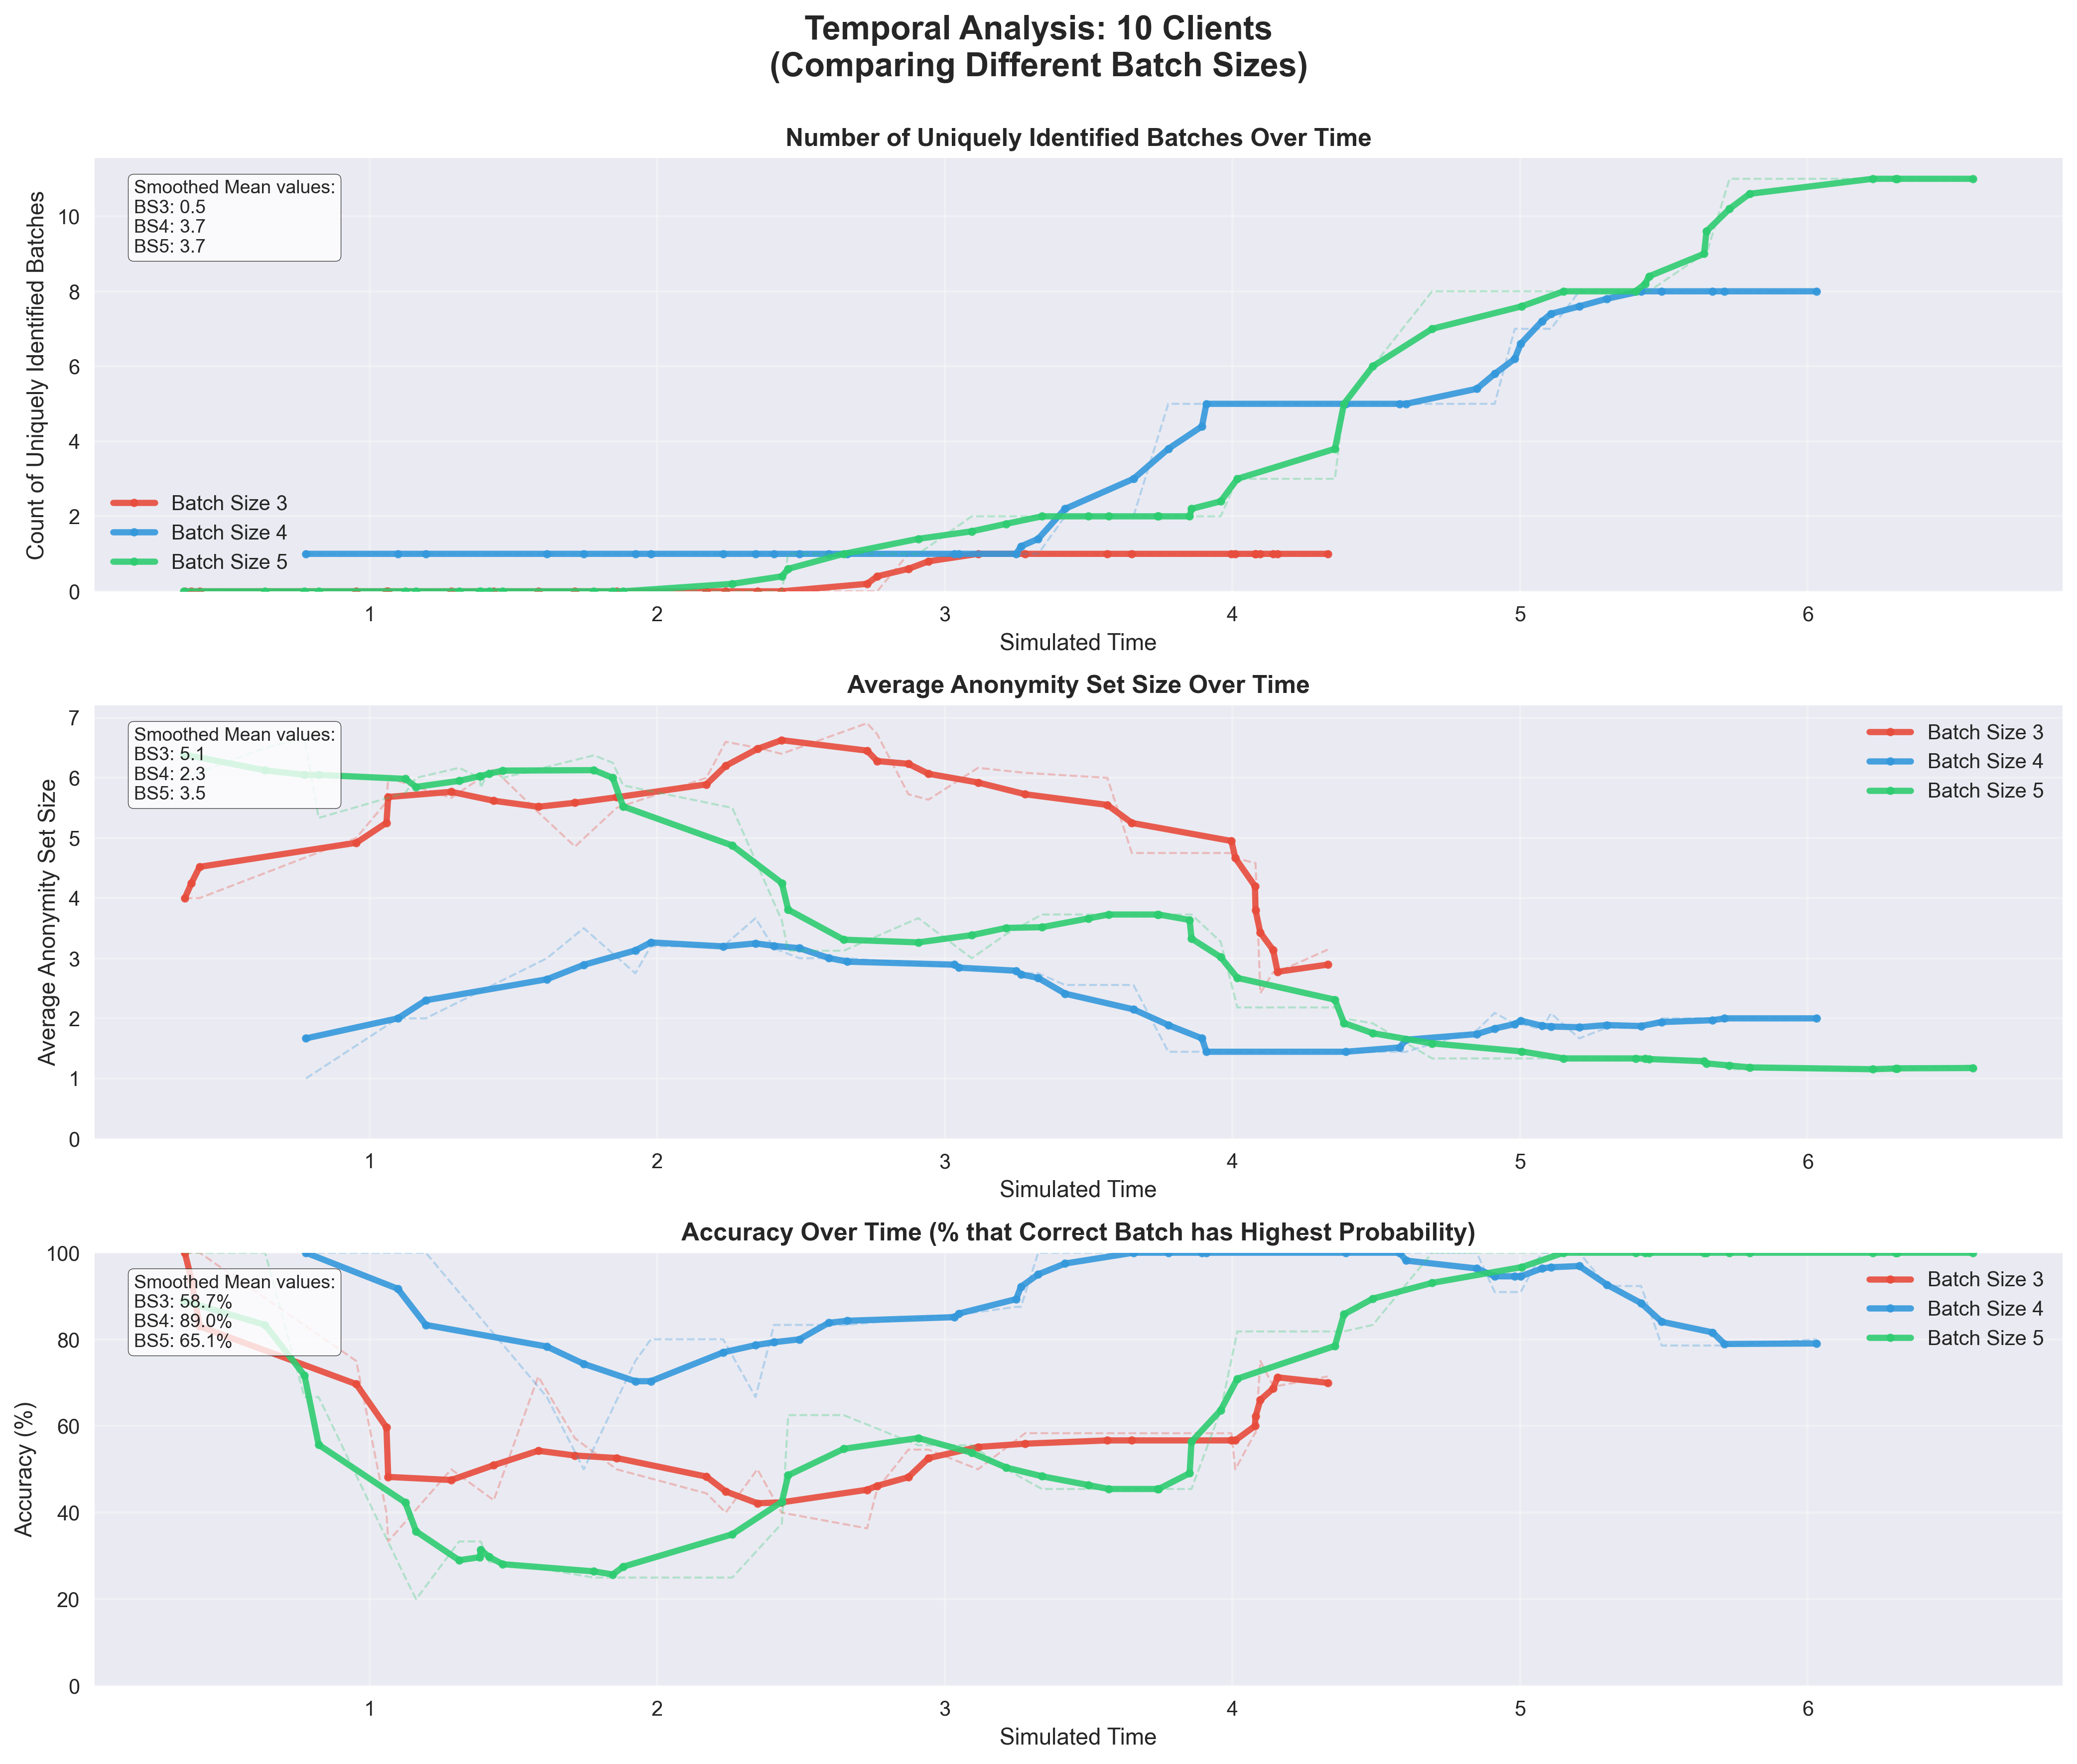
\includegraphics[width=\textwidth]{diagrams/temporal_5_smoothed_10_clients.png}
%     \caption{10 clients}
%     \label{fig:temporal_10}
% \end{minipage}
% \hfill
% \begin{minipage}{0.32\textwidth}
%     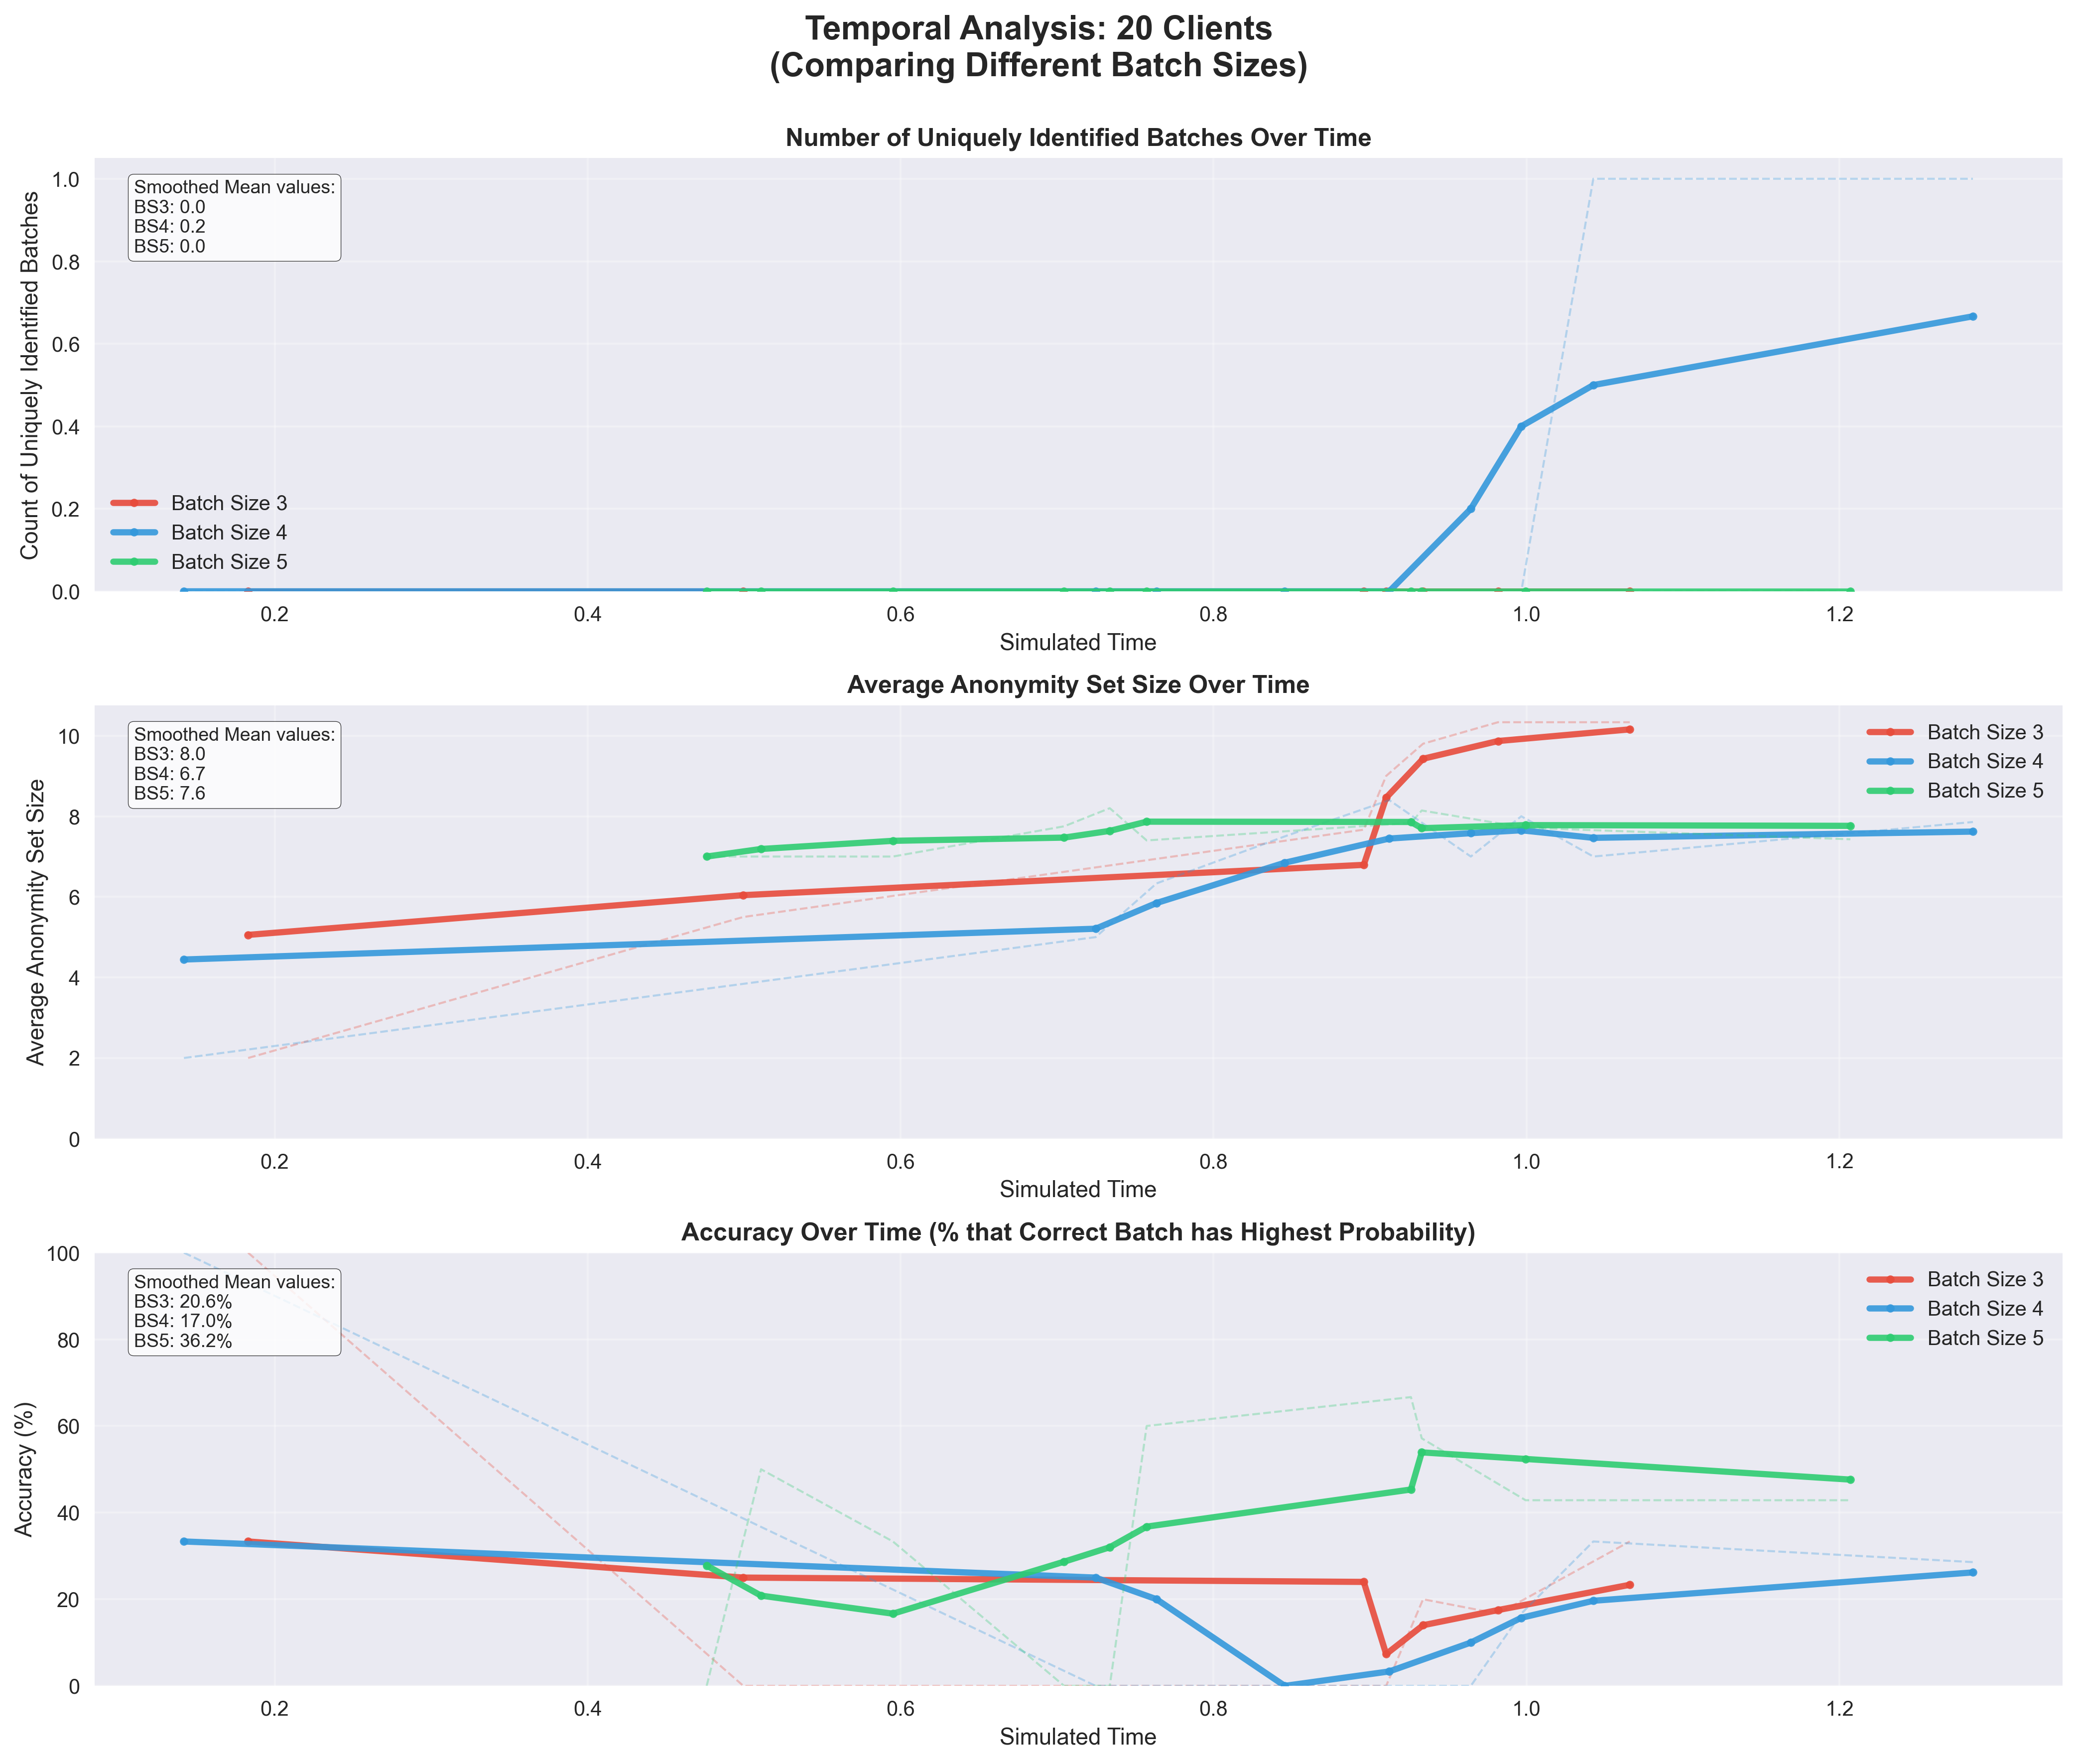
\includegraphics[width=\textwidth]{diagrams/temporal_5_smoothed_20_clients.png}
%     \caption{20 clients}
%     \label{fig:temporal_20}
% \end{minipage}
% \hfill
% \begin{minipage}{0.32\textwidth}
%     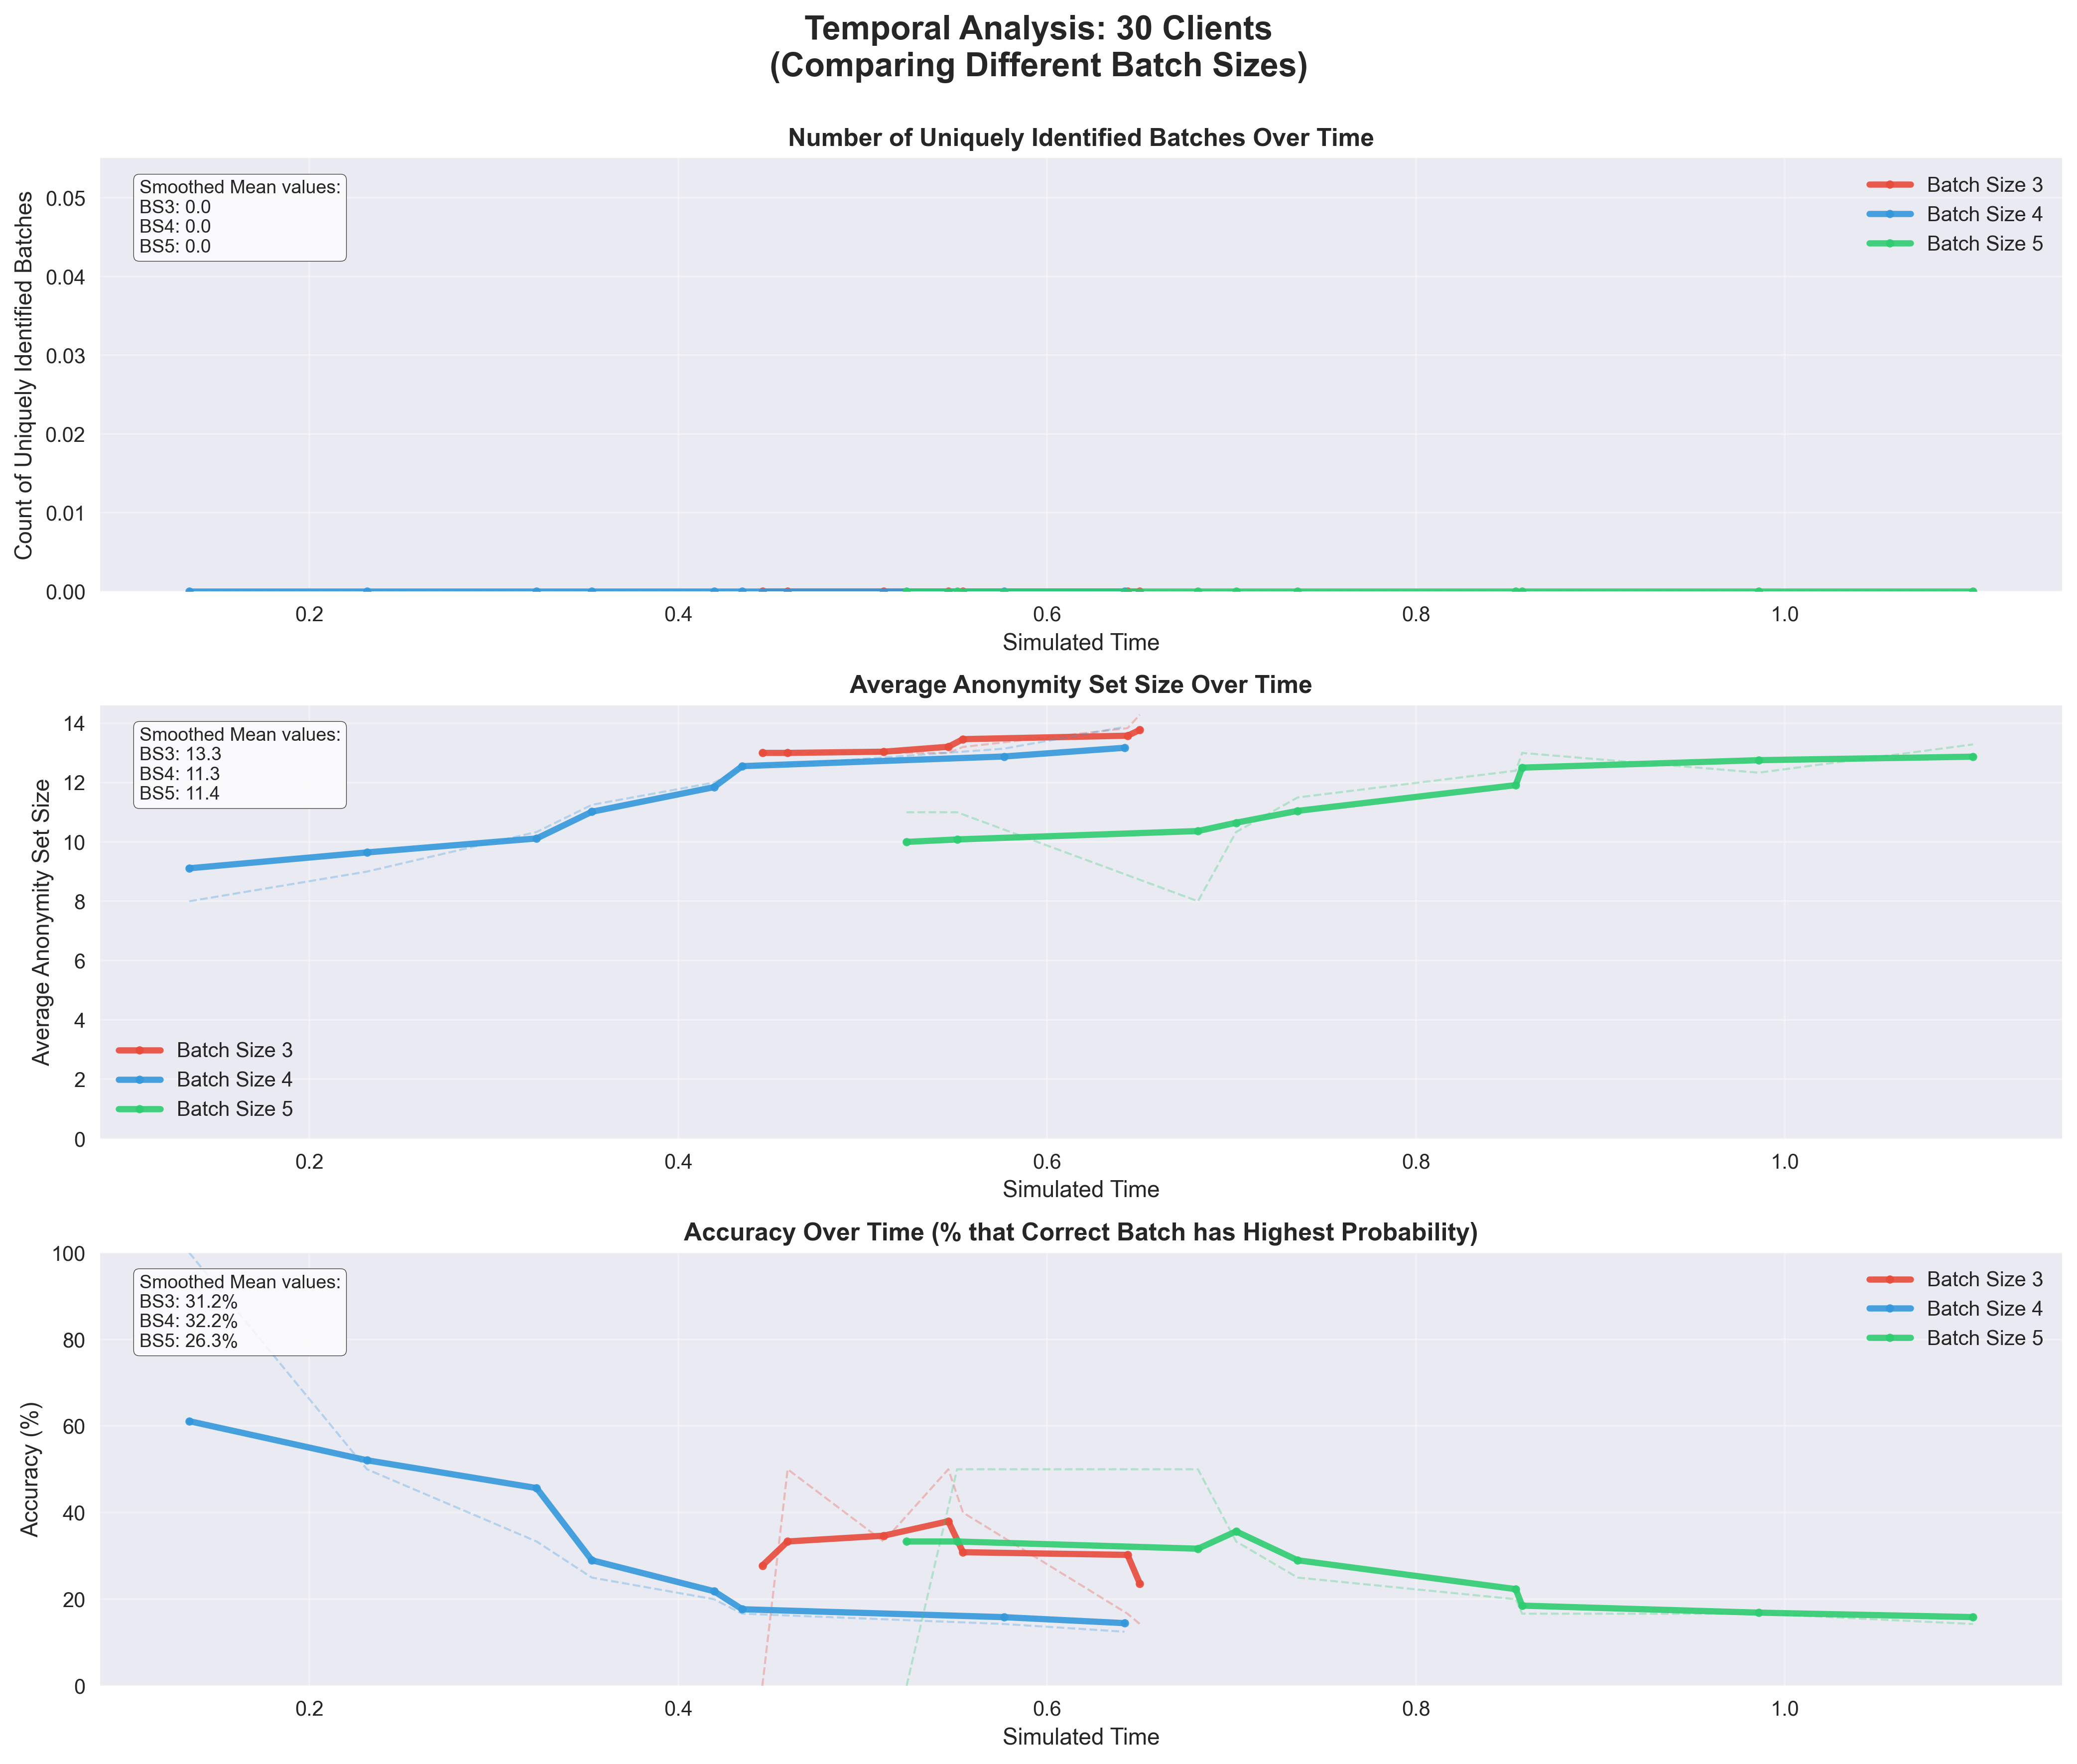
\includegraphics[width=\textwidth]{diagrams/temporal_5_smoothed_30_clients.png}
%     \caption{30 clients}
%     \label{fig:temporal_30}
% \end{minipage}
% \caption{Temporal analysis across different client populations}
% \label{fig:temporal_all}
% \end{figure*}

\begin{figure*}[!htb]
\centering
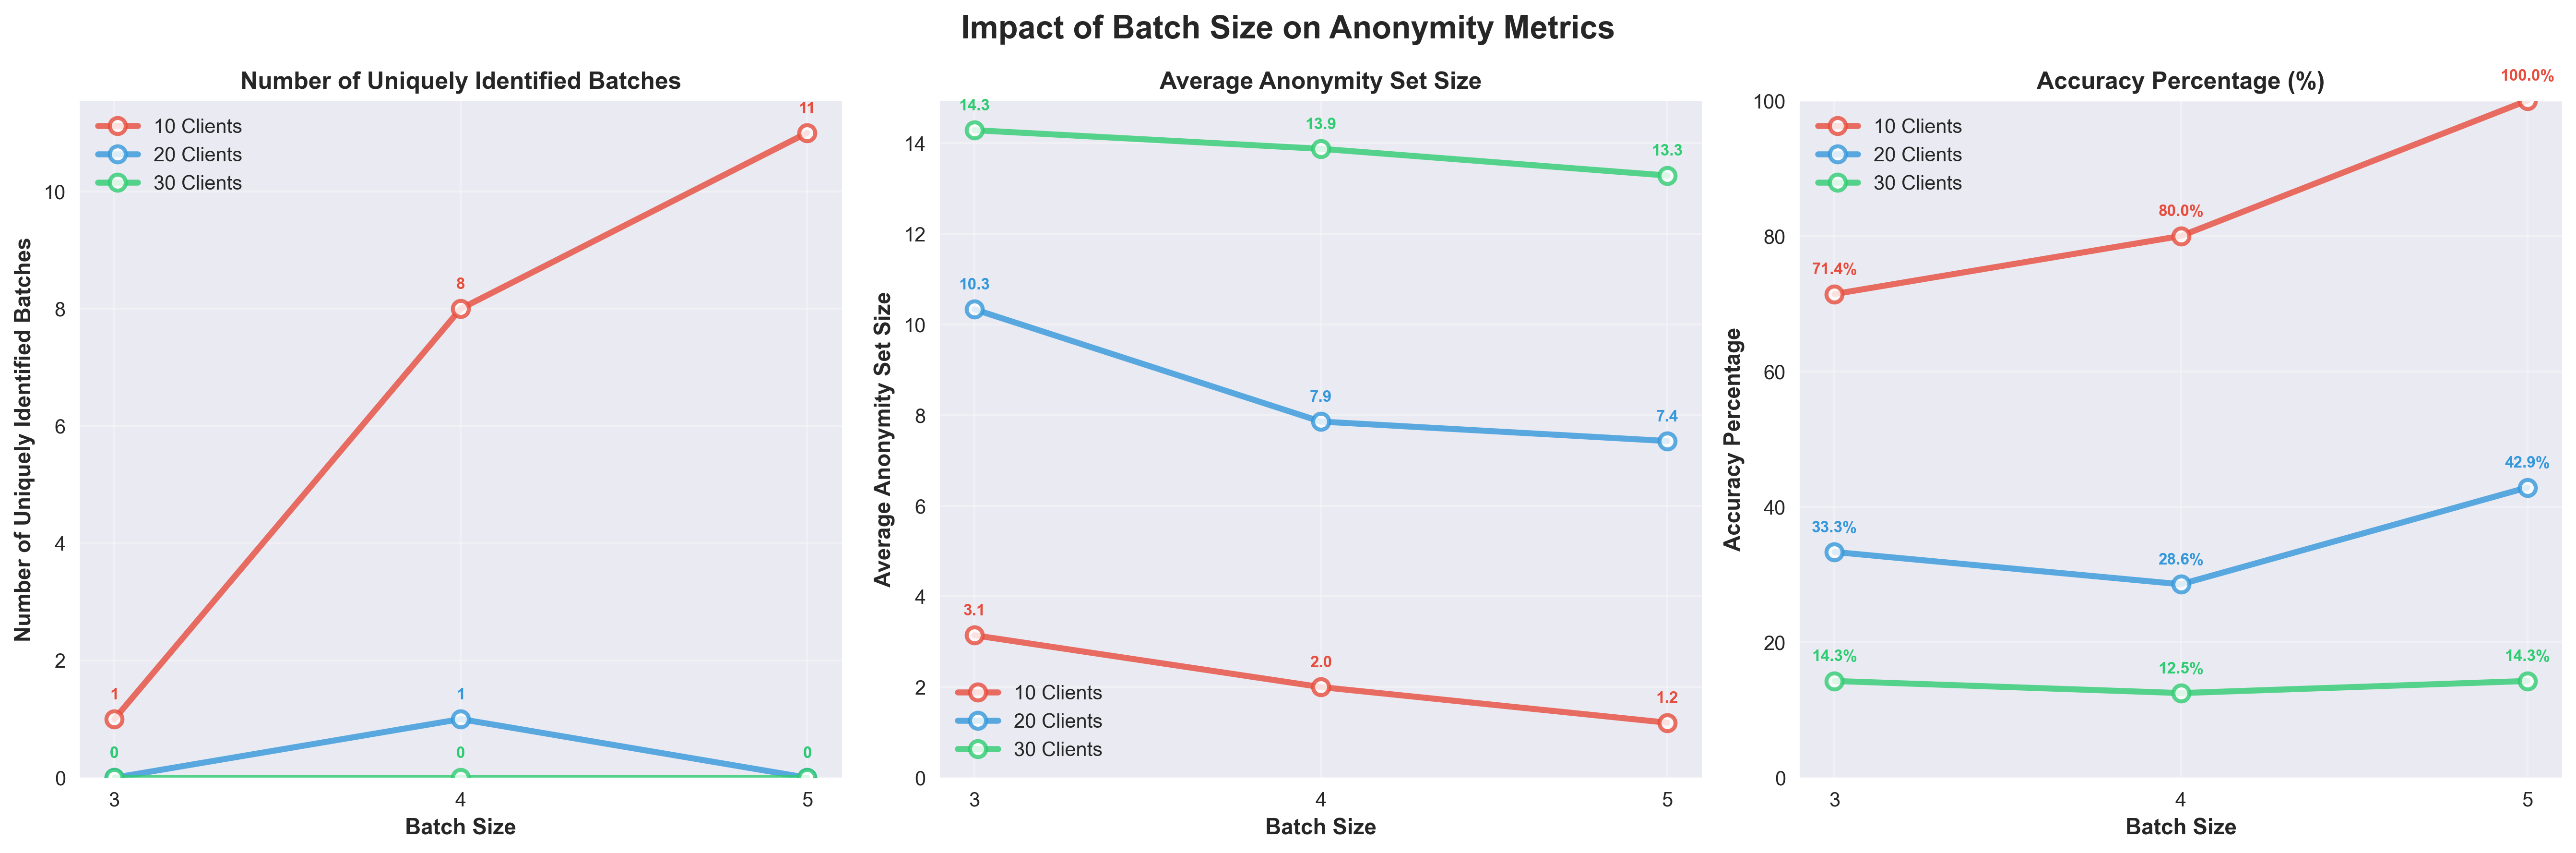
\includegraphics[width=\textwidth]{diagrams/batch_size_analysis_combined.png}
\caption{Impact of batch size on various anonymity metrics across 
different numbers of clients (10, 20, and 30 clients). 
The plots show how batch size affects the number of uniquely 
identified batches, average anonymity set size, and accuracy percentage.}
\label{fig:batchsize_analysis}
\end{figure*}

\begin{figure*}[!htb]
\centering
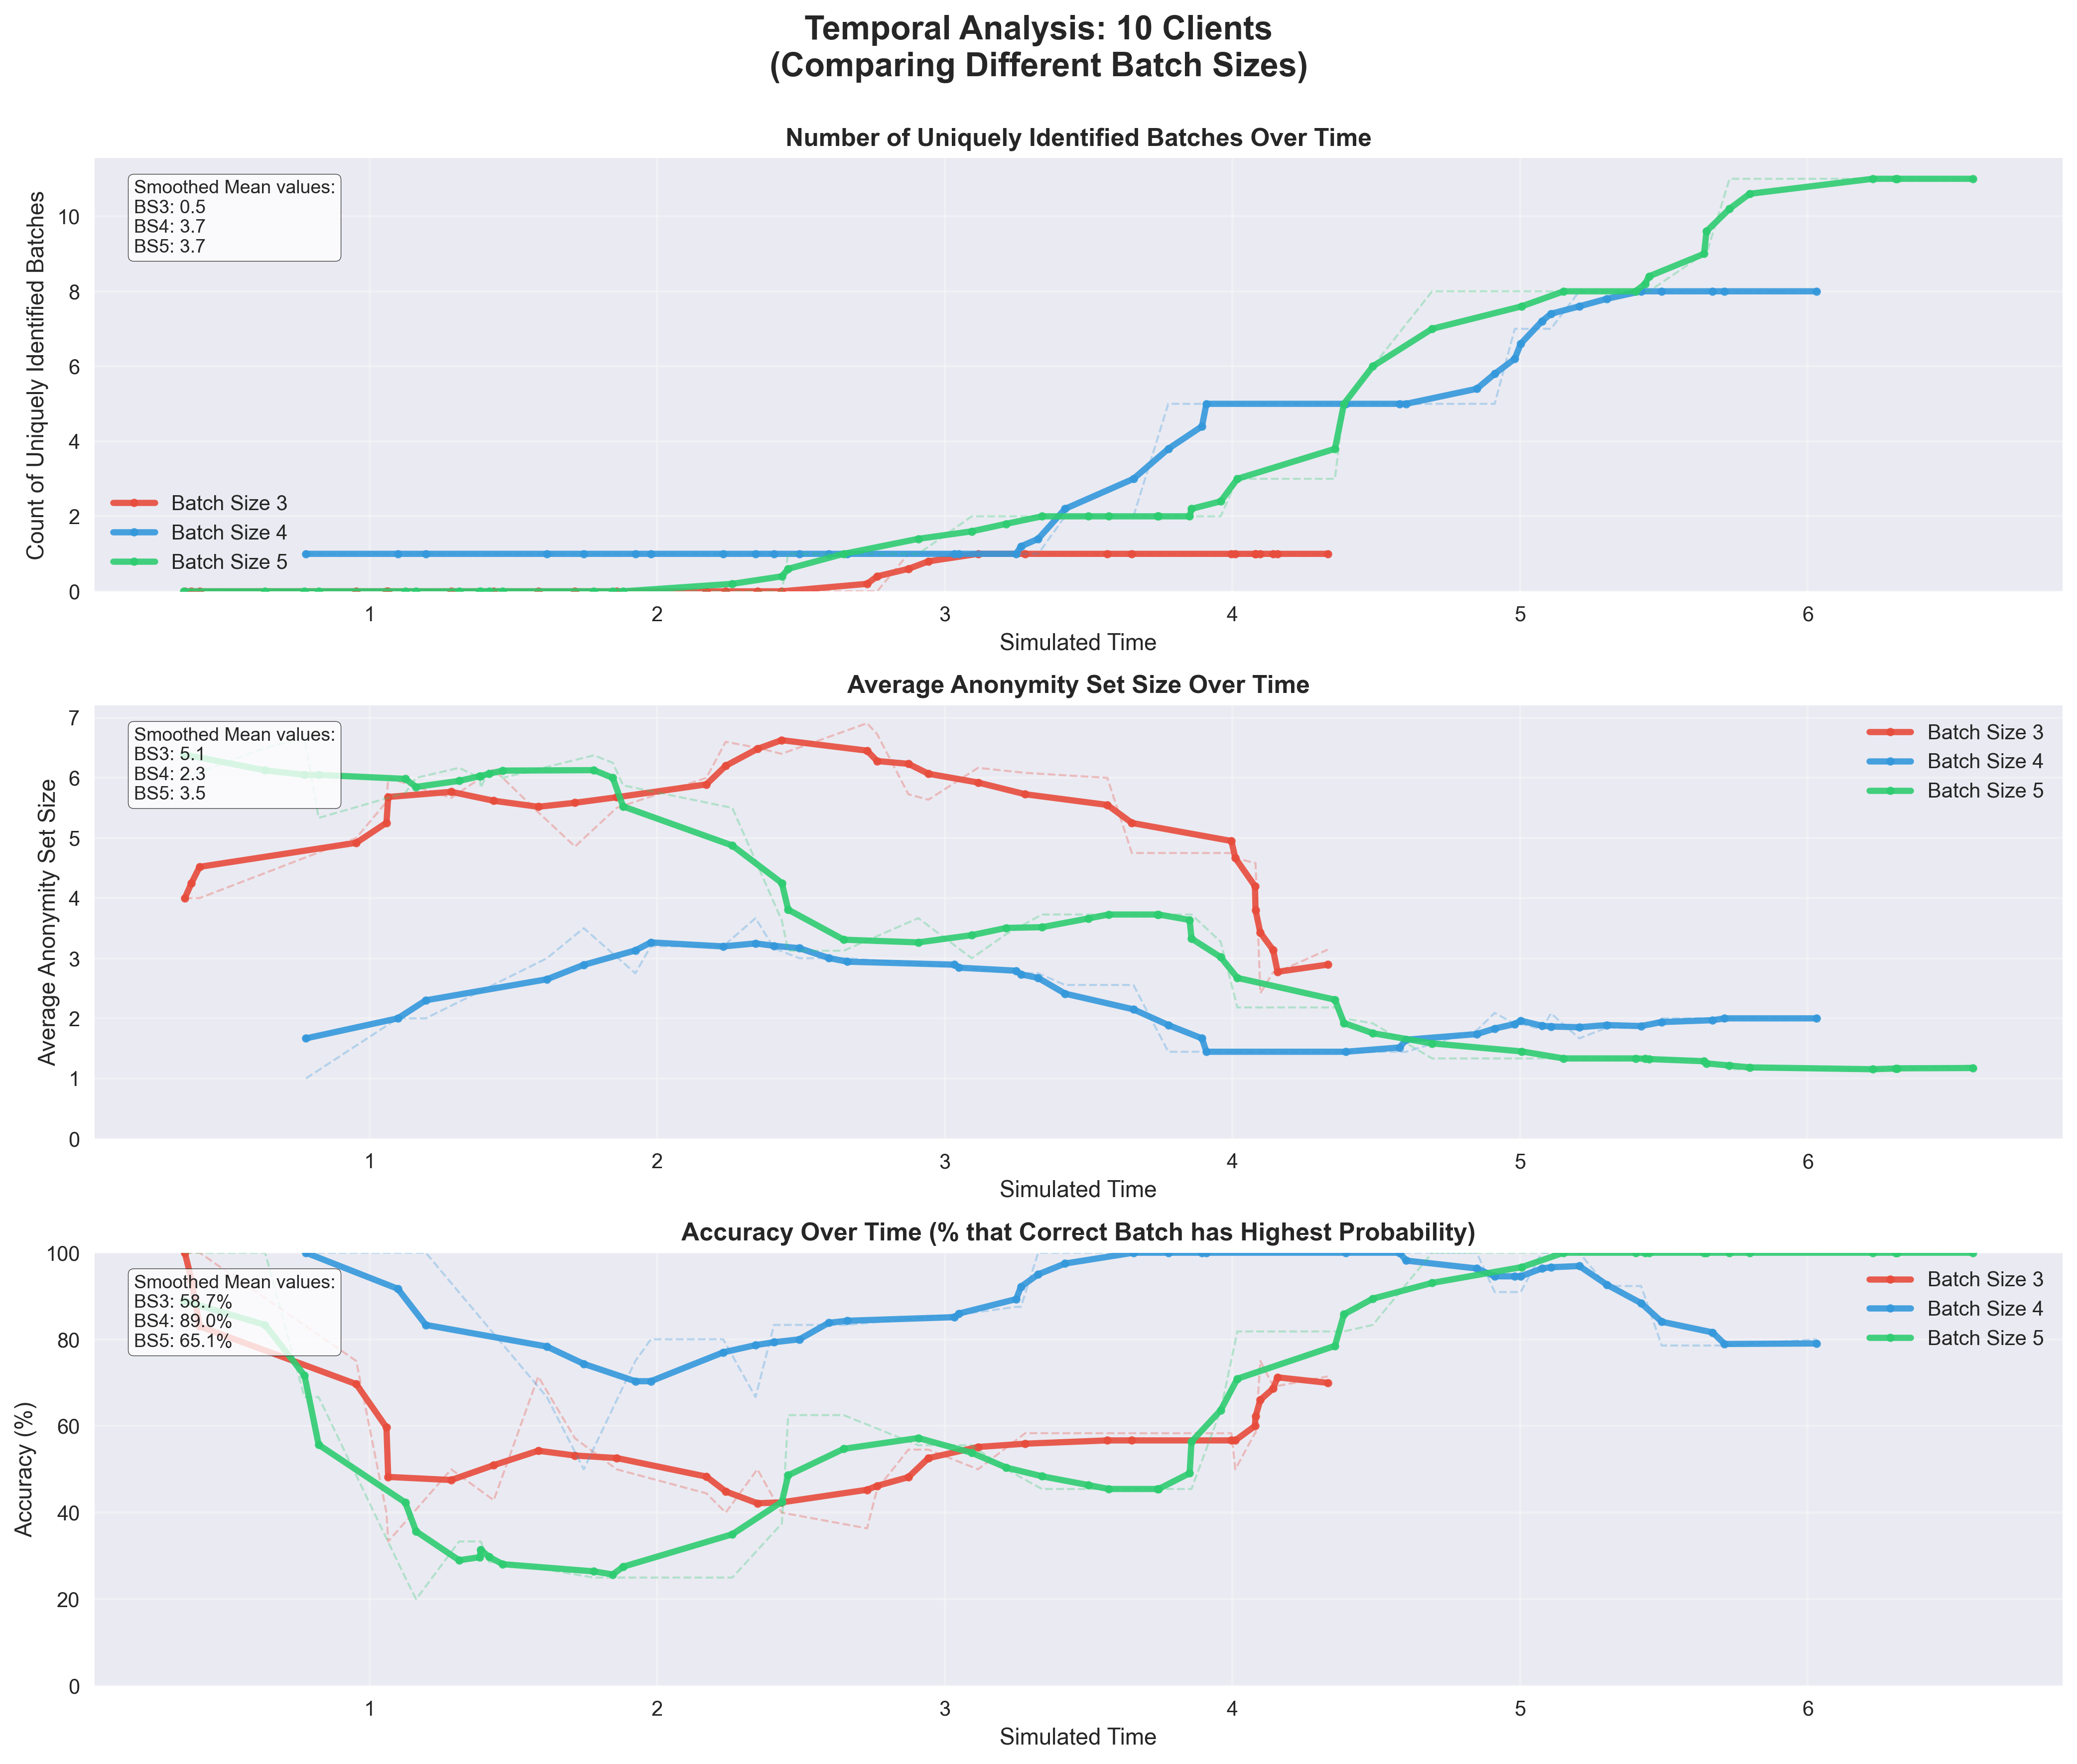
\includegraphics[width=\textwidth]{diagrams/temporal_5_smoothed_10_clients.png}
\caption{Impact of batch sizes when number of clients is 10}
\label{fig:temporal_analysis_10}
\end{figure*}

\begin{figure*}[!htb]
\centering
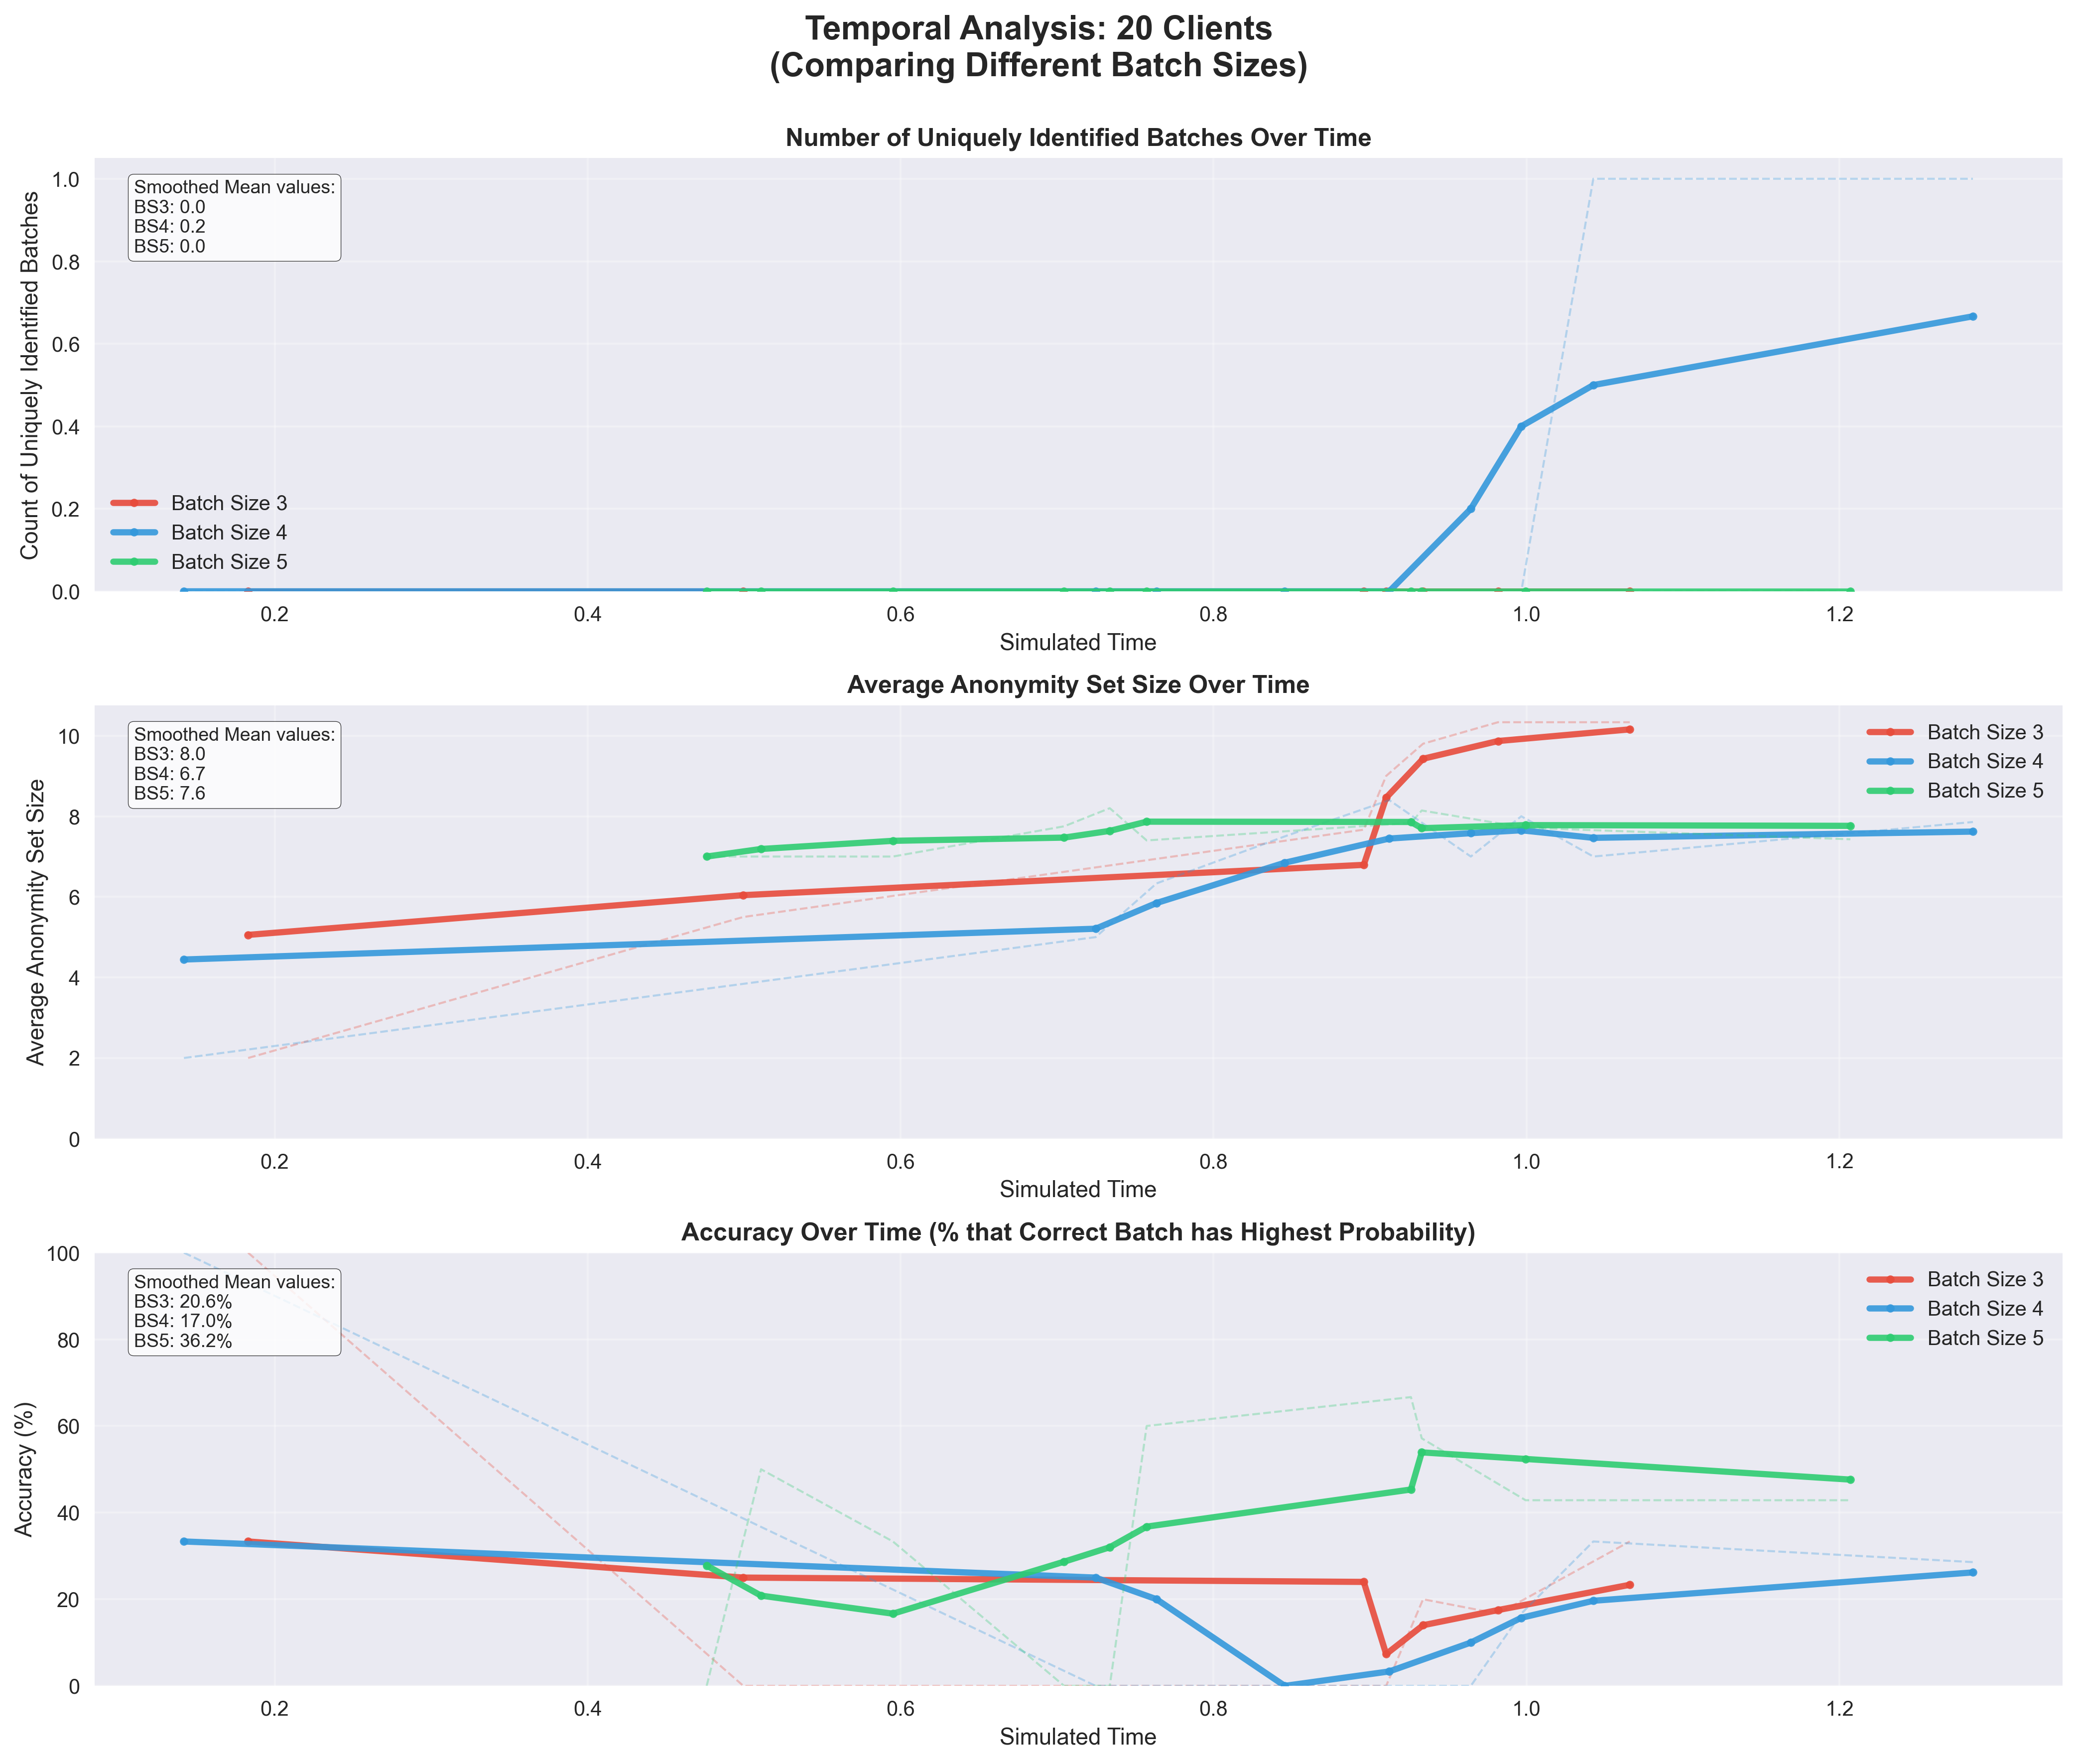
\includegraphics[width=\textwidth]{diagrams/temporal_5_smoothed_20_clients.png}
\caption{Impact of batch sizes when number of clients is 20}
\label{fig:temporal_analysis_20}
\end{figure*}

\begin{figure*}[!htb]
\centering
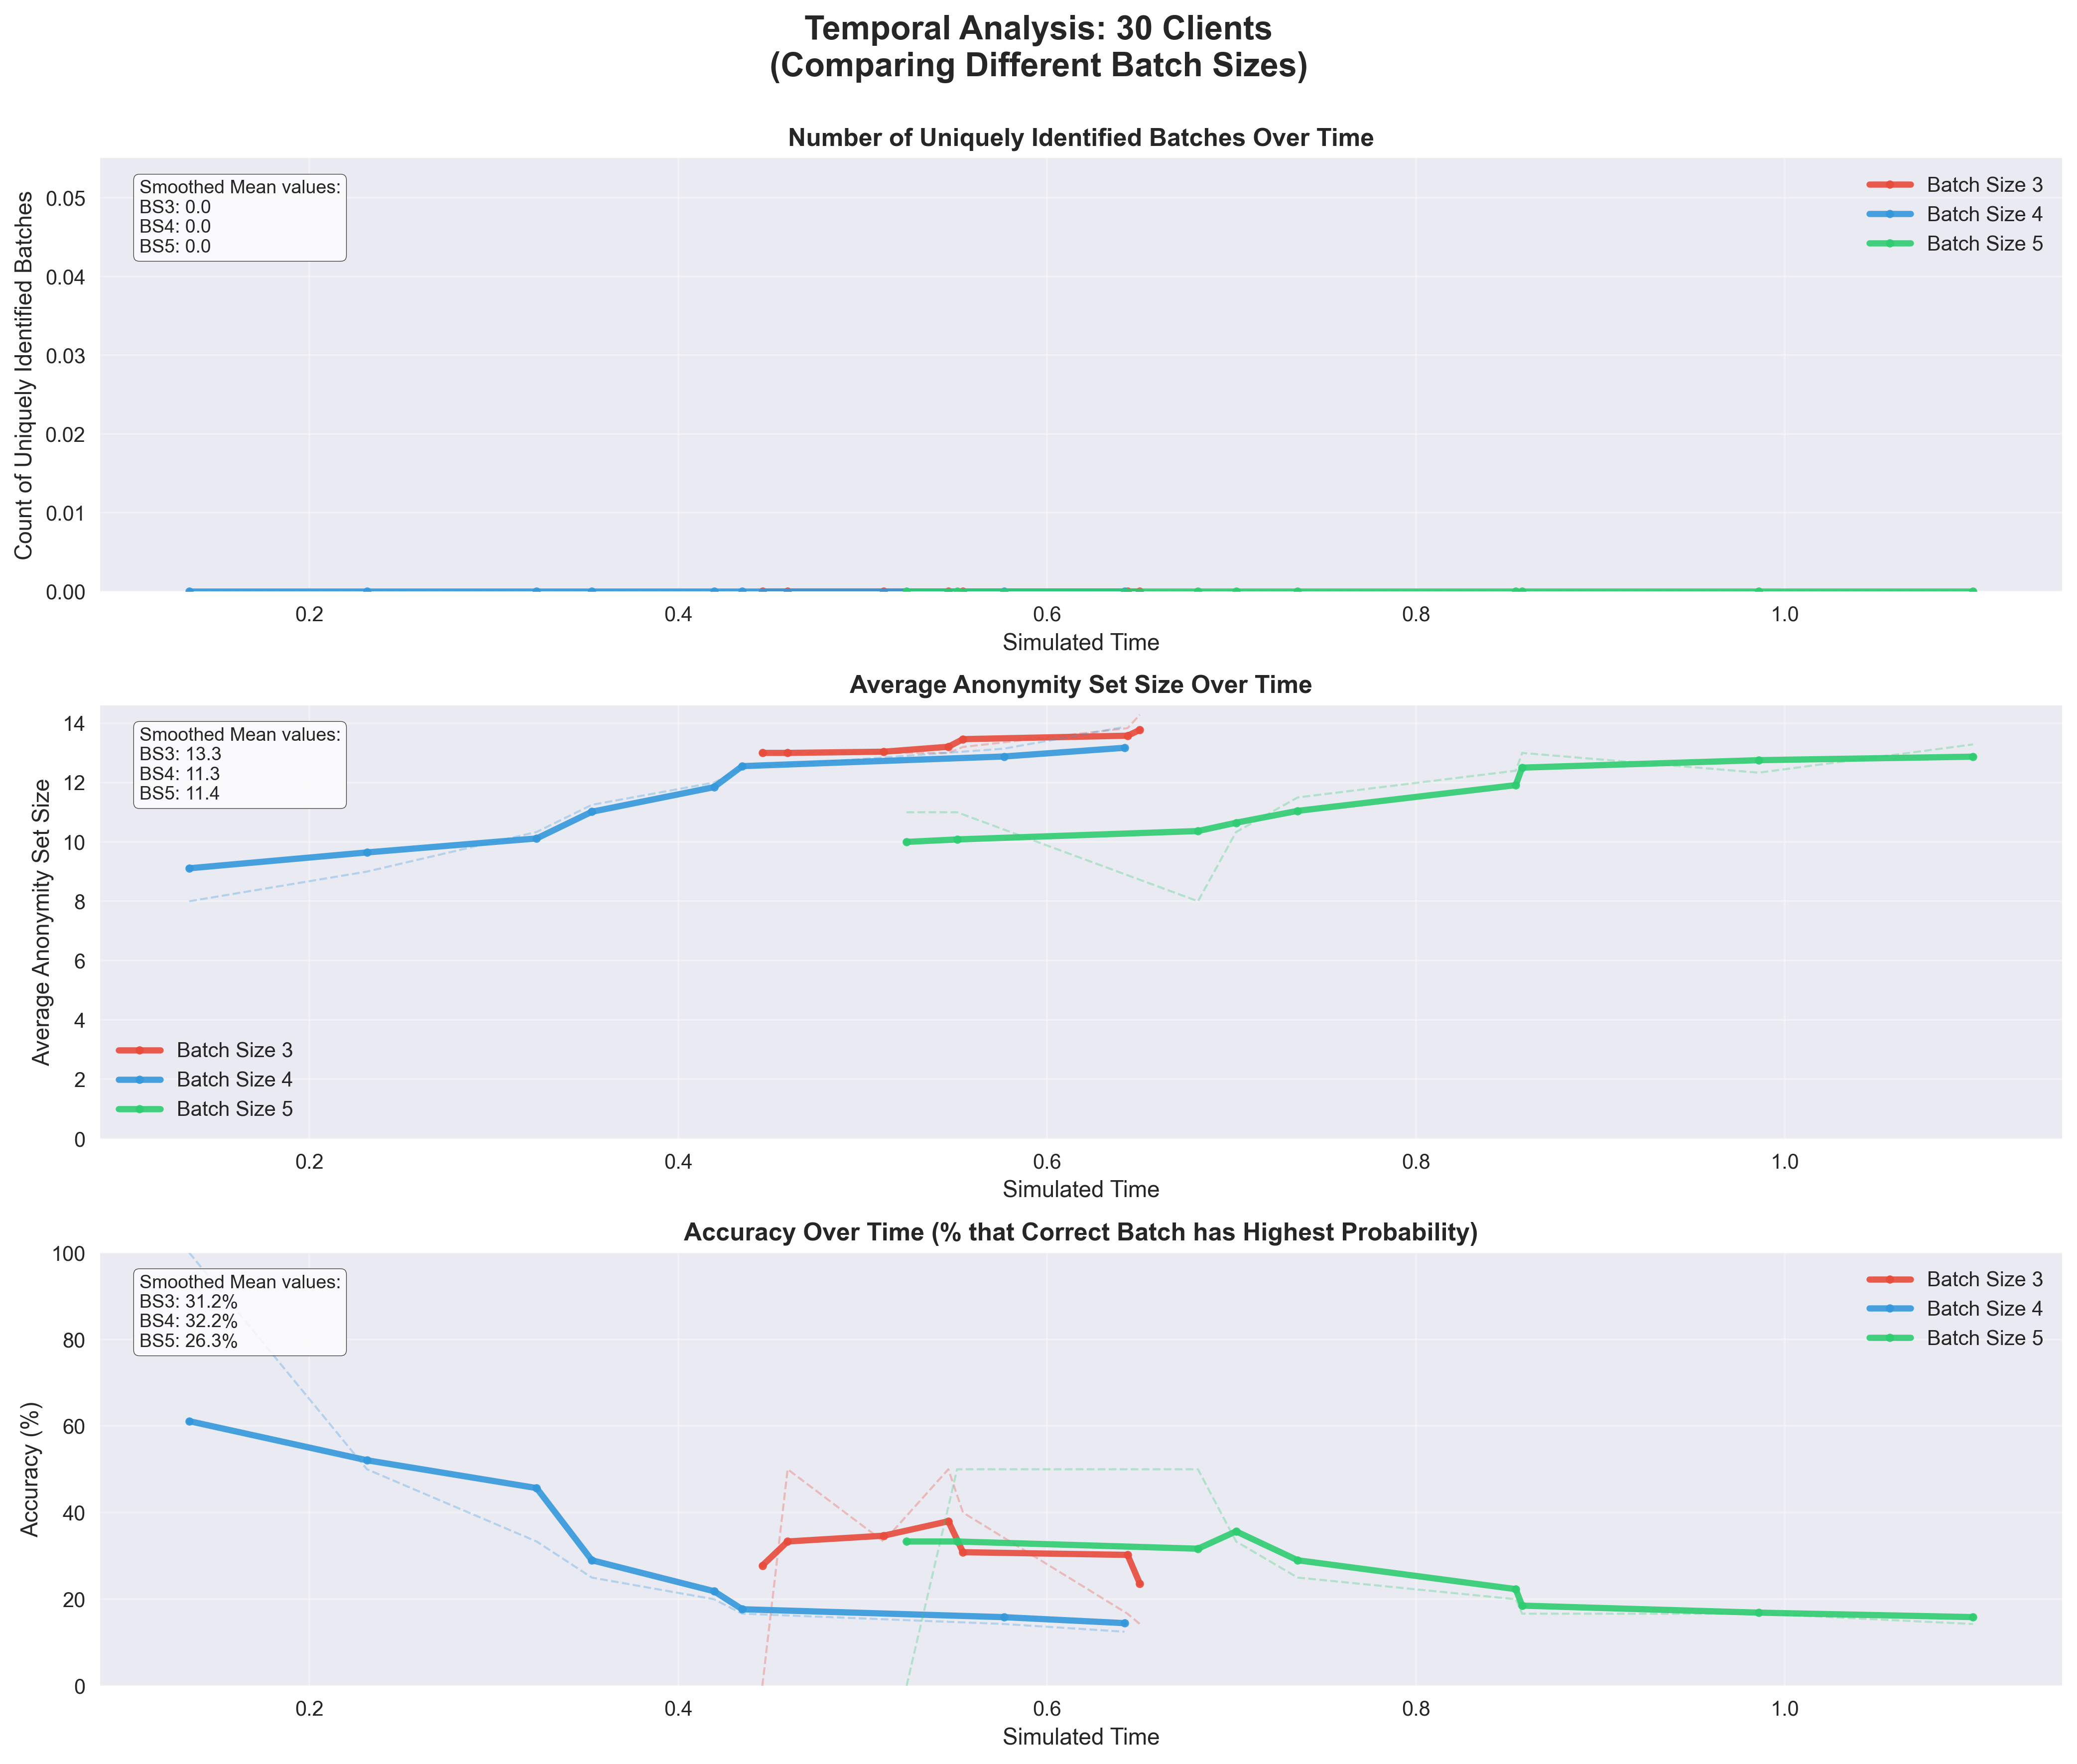
\includegraphics[width=\textwidth]{diagrams/temporal_5_smoothed_30_clients.png}
\caption{Impact of batch sizes when number of clients is 30}
\label{fig:temporal_analysis_30}
\end{figure*}

\begin{figure*}[!htb]
\centering
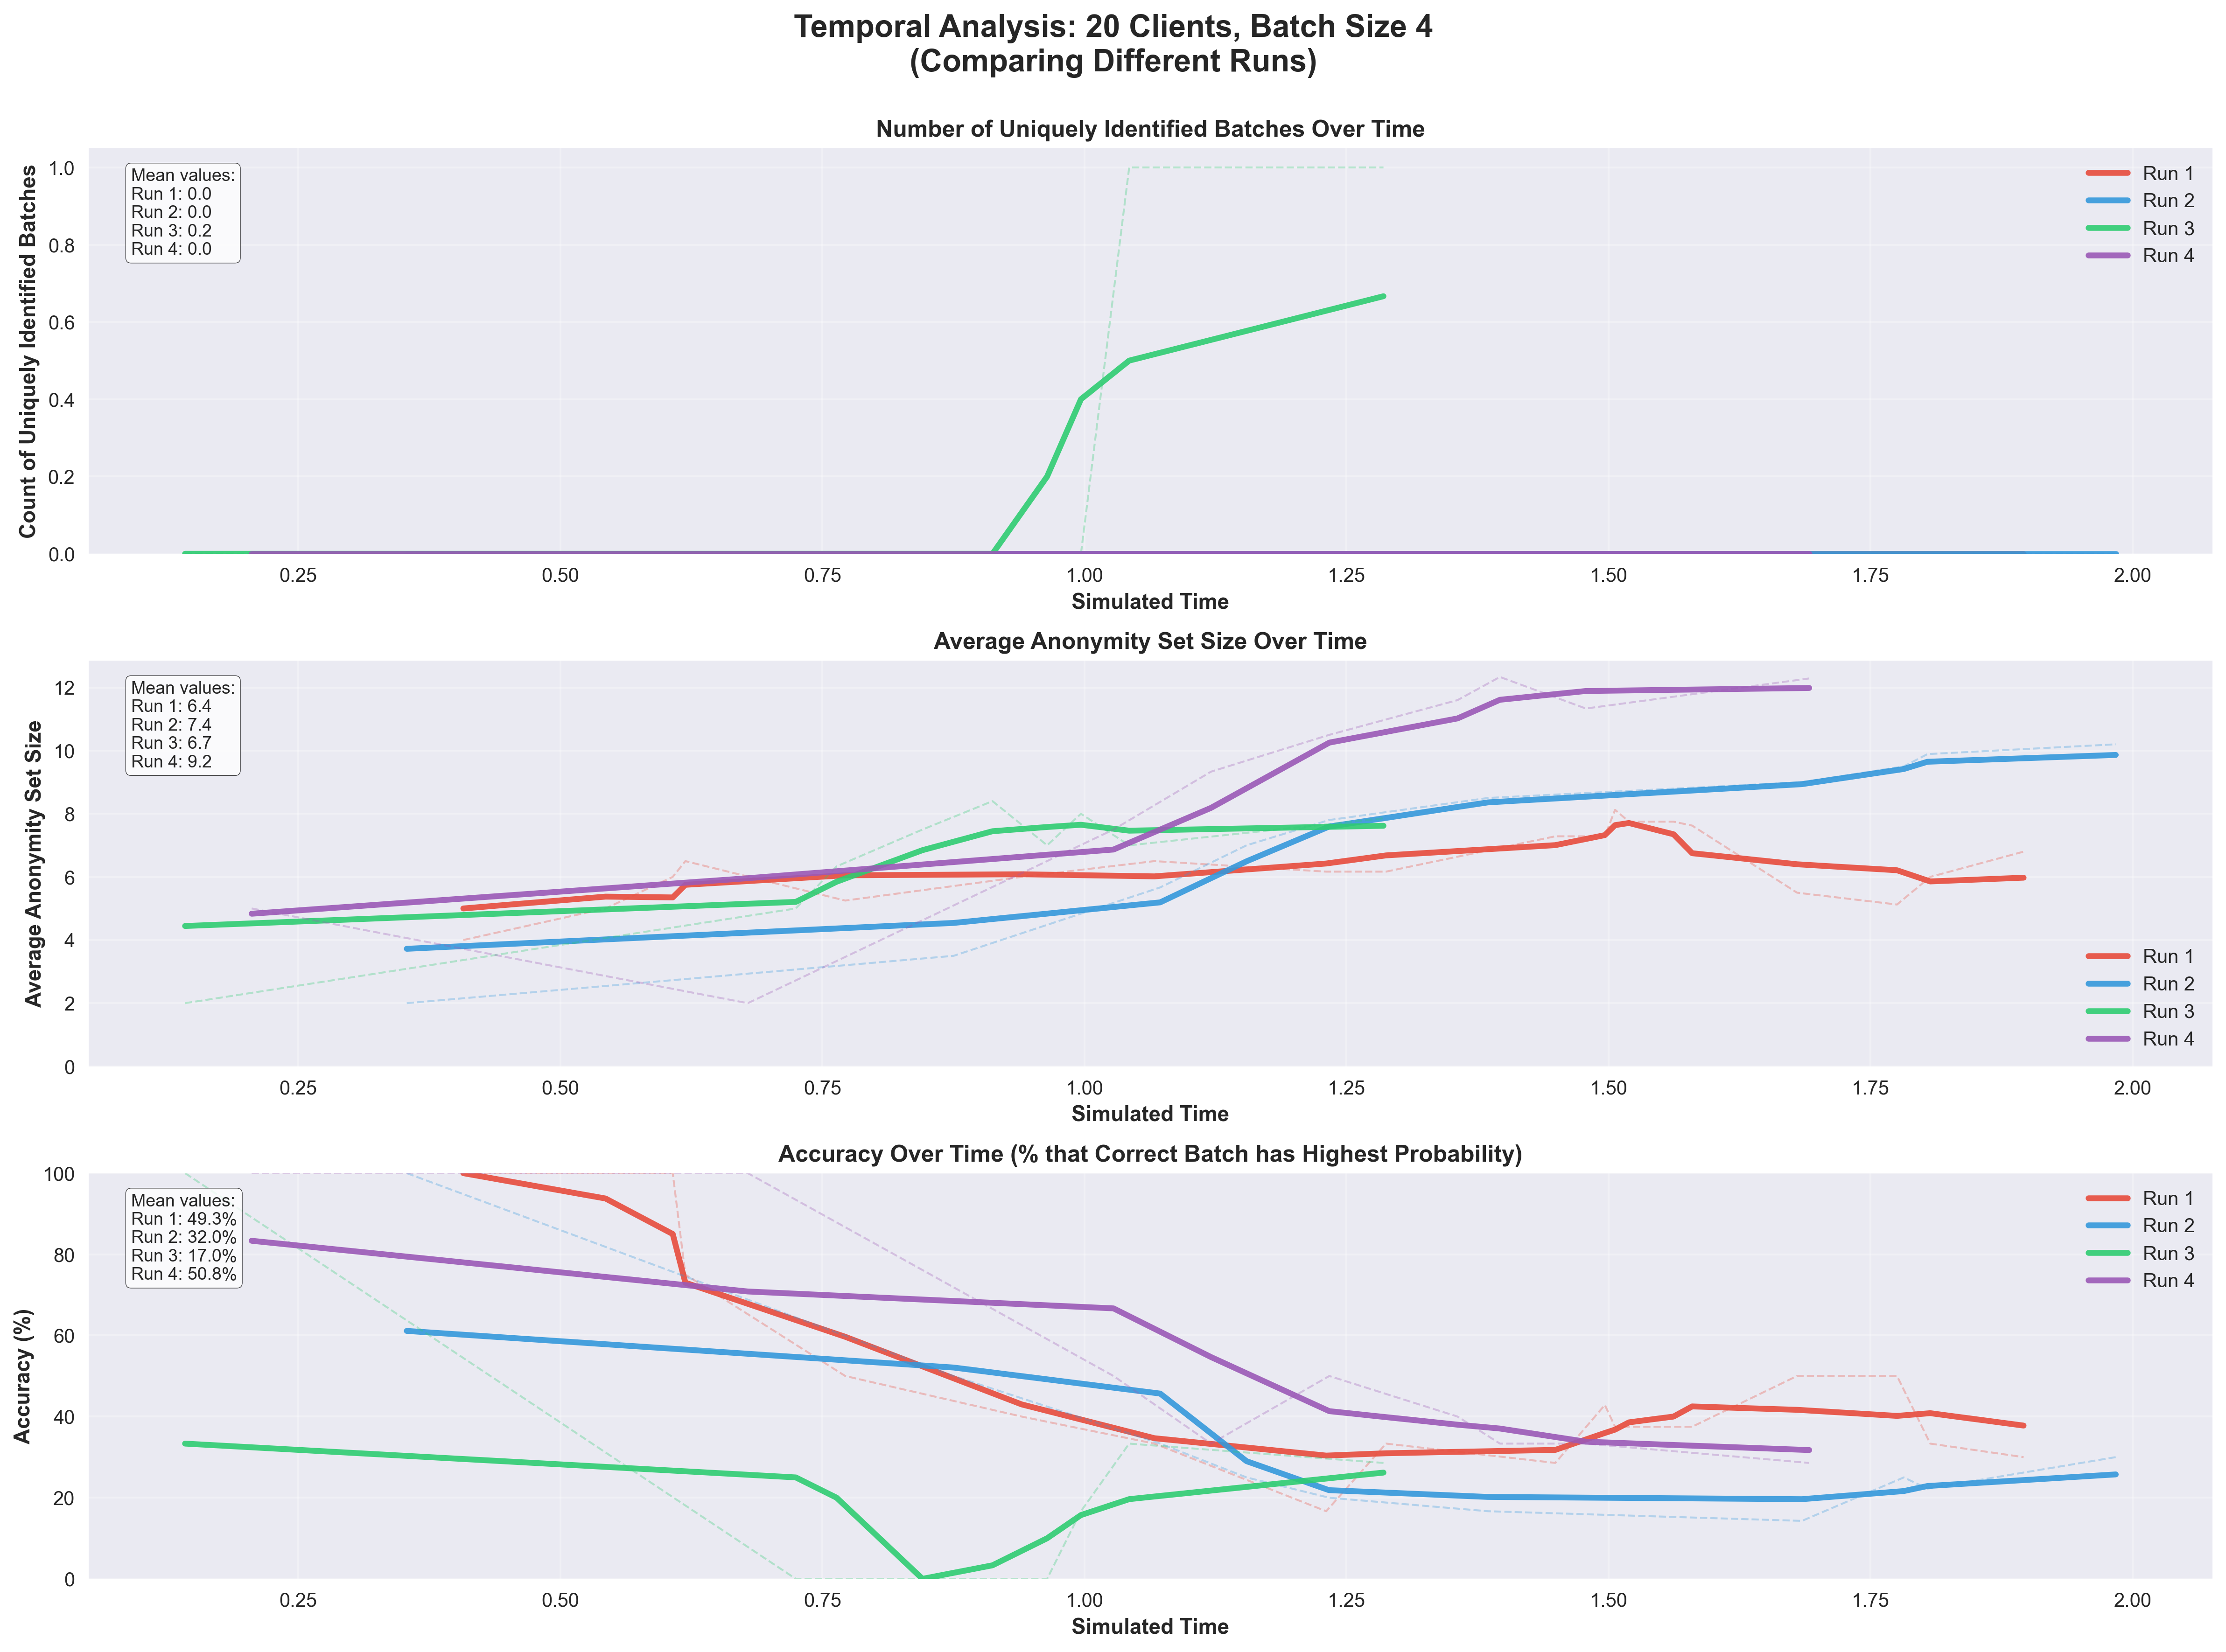
\includegraphics[width=\textwidth]{diagrams/temporal_20client_4batch_runs.png}
\caption{Comparison of 20 client 4 batch runs}
\label{fig:temporal_analysis_20_4_runs}
\end{figure*}

\subsection{Conclusion}
% \textbf{Conclusion:} 
It is important to note that due to computational limitations 
and the exponential complexity of the batch matching algorithm, 
our evaluation is based on a limited set of experimental runs. 
The patterns observed in this study should be interpreted with 
caution, as they represent only a small sample of the possible 
parameter space.

The computational complexity of enumerating all valid permutations 
scales poorly with both the number of clients and batch size, 
limiting our ability to conduct extensive statistical analysis. 
Additionally, the single-run approach for most configurations 
prevents us from establishing statistical significance or 
confidence intervals for our observations.

Future work should focus on developing more efficient algorithms 
that can handle larger parameter spaces and enable comprehensive 
statistical evaluation of anonymity guarantees under various 
operational conditions.

\end{document}